% !TeX encoding = UTF-8
% !TeX program = pdflatex
\documentclass[english,noexaminfo,a4paper,oneside, binding = 0.6cm]{sapthesis}
%remove "english" for a thesis written in Italian
%Bachelor's (laurea triennale) thesis : Lau 
%Master's (laurea specialistica) thesis: LaM 
%PhD's thesis: PhD 
%\usepackage[italian]{babel} %use this package for a thesis written in Italian
\usepackage[utf8]{inputenc}
\usepackage{indentfirst}
\usepackage{dsfont}
\usepackage{microtype}
\usepackage{colortbl}
\usepackage[table]{xcolor}
\definecolor{lightgray}{gray}{0.9} % 0.9 is very light, 0.1 is very dark
\usepackage{booktabs} % For professional lines
\usepackage{enumitem}
%\usepackage{chemformula}
%\usepackage{setspace}
%\usepackage{yfonts,color}F
%\usepackage{siunitx}
%\usepackage{comment}
%\usepackage{multirow}
%\usepackage{varioref}
%\usepackage[bottom]{footmisc}
%\usepackage{wrapfig}
%\usepackage{float}
%\usepackage{type1cm}
\usepackage{lettrine}
\linespread{0.9}
%\usepackage{chngcntr}
\usepackage{graphicx}
\usepackage{subcaption}
\usepackage[nottoc, notlof, notlot]{tocbibind}
%\onehalfspacing
%\counterwithout{footnote}{chapter}
\usepackage{microtype}
\usepackage[utf8]{inputenc}
\usepackage{listings}
\usepackage{xcolor}
\usepackage{amsfonts}
\usepackage{amsmath}
\usepackage{amssymb} % Added for \varnothing and \mathcal
\usepackage[linesnumbered,ruled,vlined]{algorithm2e}
\usepackage[hidelinks]{hyperref}
\usepackage[nameinlink]{cleveref}
\usepackage{placeins}
\setlist[enumerate,1]{start=0} % only outer nesting level
\hypersetup{
			hyperfootnotes=true,			
			bookmarks=true,			
			colorlinks=true,
			linkcolor=red,
            linktoc=page,
			anchorcolor=black,
			citecolor=red,
			urlcolor=blue,
			pdftitle={Evaluation of Statistical Methods for Generative Password-guessing models},
			pdfauthor={Roberto Di Rosa},
			pdfkeywords={thesis, sapienza, roma, university}
 }

\title{Evaluation of Statistical Methods for Generative Password-guessing models}
\author{Roberto Di Rosa}
\IDnumber{2043388}
\course{Informatica}
\courseorganizer{Facolt\`a di Ingegneria dell'informazione, informatica e statistica}
\submitdate{2025/2026}
\copyyear{2025}
\advisor{Prof. De Gaspari}
\coadvisor{}
\authoremail{dirosa.2043388@studenti.uniroma1.it}
%\examdate{xx December 2025}
%\examiner{Prof. ...} \examiner{Prof. ...} \examiner{Prof. ...}  \examiner{Prof. ...} % \examiner{Prof. ...} \examiner{Prof. ...}  \examiner{Prof. ...} 

%we refer to http://ctan.mirrorcatalogs.com/macros/latex/contrib/sapthesis/sapthesis-doc.pdf for an exhaustive description of the sapthesis documentclass.
\definecolor{codegreen}{rgb}{0,0.6,0}
\definecolor{codegray}{rgb}{0.5,0.5,0.5}
\definecolor{codepurple}{rgb}{0.58,0,0.82}
\definecolor{backcolour}{rgb}{0.95,0.95,0.92}
% --- Doom One Light Color Definitions ---
% (Add this to your preamble)
\definecolor{doomBack}{RGB}{250, 250, 250}     % #fafafa
\definecolor{doomComment}{RGB}{156, 156, 156}   % #9c9c9c
\definecolor{doomKeyword}{RGB}{198, 120, 221}   % #c678dd (Purple/Magenta)
\definecolor{doomString}{RGB}{152, 195, 121}    % #98c379 (Green)
\definecolor{doomNumber}{RGB}{209, 154, 102}    % #d19a66 (Orange)
\definecolor{doomDefault}{RGB}{77, 77, 77}      % #4d4d4d (Default Text)
% Setup section. -----------------------------------|


\lstdefinestyle{pythonstyle}{
  language=Python,
  basicstyle=\ttfamily\small,
  backgroundcolor=\color{doomBack}, 
  commentstyle=\color{doomComment},
  keywordstyle=\color{doomKeyword},
  numberstyle=\tiny\color{doomNumber},
  stringstyle=\color{doomString},
  basicstyle=\ttfamily\footnotesize\color{doomDefault},
  breakatwhitespace=false,         
  breaklines=true,                 
  captionpos=b,                    
  keepspaces=true,                 
  numbers=left,                    
  numbersep=8pt,                  
  showspaces=false,                
  showstringspaces=false,
  showtabs=false,                  
  tabsize=2
}


\begin{document}

\frontmatter
\maketitle

\begin{abstract}
  TODO
\end{abstract}

\tableofcontents

\mainmatter
\chapter{Introduction}
\lettrine[lines=2, findent=3pt, nindent=0pt]{I}{}n the field of probabilistic password-guessing models, evaluating a password's resistance to guessing attacks requires estimating its \textit{guess number}.
This practice is very important since passwords are and will be for the foreseable future the most common human authentication method\cite{}, and humans tend to use weak patterns for simplicity reasons\cite{}, therefore research in this field has focused on how to define if a password is secure or not, so that we can distringuish a weak password from a strong one in a reliable manner.
We do this by measuring the guessability of a password, the higher the guessability the more difficult it will be to guess a password therefore rendering it much more secure.
To do this we have to study the POV of the attackers, this is what MAYA~\cite{ref:maya} does, it defines an extensible framework for testing Models on this matter. 
The guess number represents the expected number of attempts an attacker would need to generate or match a specific password.
In recent years, there has been a rise in Generative Password-guessing Models some of which can be seen in MAYA such as: FLA~\cite{ref:fla}, PassGAN~\cite{ref:passgan}, PassGPT~\cite{ref:passgpt}, PLRGAN~\cite{ref:pasquini}, and the PassLLM framework~\cite{ref:pwdguessllm}. These models aim to learn complex human password patterns to improve guessing efficiency. The standard method for evaluating these models involves generating a \textit{top-k} list of probable passwords and comparing them against a testing dataset.
However, this evaluation approach introduces a significant computational challenge. Generating and maintaining this \textit{top-k}\footnote{Not all models generate the top-k(e.g. GAN like models), only explicit models do this.} list requires processing an enormous set of passwords, which imposes severe memory demands. As noted in MAYA~\cite{ref:maya} and FLA~\cite{ref:fla}, this memory bottleneck often necessitates high-performance computing (HPC) resources, making standard evaluation intractable.
One potential alternative is to use Monte Carlo estimation~\cite{ref:dellamico} to approximate model performance. However, the accuracy of Monte Carlo estimation has not been rigorously proven for all ranges of guess numbers, particularly for rare passwords.
Currently, the MAYA implementation of the FLA \textit{get\_topk} routine suffers from significant "object overhead." This inefficiency renders the model un-evaluatable in standard environments (e.g., machines with less than 200 GB of RAM) when attempting sample sizes of $N=5.0\cdot 10^8$. 
This thesis addresses this scalability limitation by replacing the standard sampling logic with a custom Heap data structure implemented in Cython. This solution eliminates the Python object overhead and achieves an $\sim87.47\%$ improvement in memory efficiency compared to the baseline implementation. Consequently, this optimization enables evaluations with sample sizes exceeding $N=5.0\cdot10^8$ on standard hardware. Furthermore, by enabling the processing of larger sample sizes, this work allows for the empirical verification of Monte Carlo estimations at a scale previously unattainable.\section{Contributions}
This allowed us to verify Monte Carlo up to $5\cdot10^8$ while using just 30GB of RAM.
\begin{itemize}
    \item An implementation of a Cython-based optimized heap item (\texttt{heap-item}), which reduces memory consumption while maintaining compatibility with Python's \texttt{heapq} module.
    \item A custom heap implementation (\texttt{heapcy}), designed to maximize performance by storing only file offsets rather than full strings, resulting in significant memory savings and faster operations.
    \item An integration of these optimizations into the MAYA framework to improve Monte Carlo rank estimation.
    \item A large-scale Monte Carlo experiment demonstrating that evaluation-estimation remains reliable up to $x = 5 \cdot 10^8$, far beyond the $10^7$ tested in the original FLA paper.
\end{itemize}
The remainder of this thesis is structured as follows. Chapter~2 presents the motivation for this work, discussing the importance of password strength evaluation and the limitations of existing sampling approaches. Chapter~3 provides background material and an overview of related work in password-guessing models and Monte Carlo estimation. Chapter~4 describes the methodology and the proposed optimizations in detail. Chapter~5 explains the experimental setup used for evaluating the new implementations. Chapter~6 presents and analyzes the results. Finally, Chapter~7 concludes the thesis and outlines directions for future research.
\chapter{Motivation}
\label{chap:2}
Human-chosen passwords remain one of the most widely used authentication mechanisms, yet they continue to exhibit significant weaknesses. Password leaks occur frequently and at large scale, enabling attackers to build increasingly accurate probabilistic models that capture human password-selection patterns. Understanding how resistant user-chosen passwords are to such guessing attacks is therefore essential both for security research and for practical password-strength meters.

Modern password-guessing models estimate the probability of strings and generate guesses in decreasing likelihood order. A password's \textit{guess number} is defined as the number of guesses an attacker would need before encountering it in this ranked list. Determining this value exactly is infeasible for models with exponentially large output spaces. Monte Carlo estimation offers a tractable alternative, providing unbiased estimates of guess numbers without requiring full enumeration.

However, Monte Carlo estimation verification imposes significant computational demands. Verification requires very large sample sizes, in the order of billions of generated passwords. Since each sample requires updating heap structures, memory footprint and sampling speed become the primary bottlenecks in frameworks such as MAYA.
Monte Carlo also has a problem when estimating low probability passwords, as demonstrated in \cite{ref:stanek}  there are ways to mitigate it, but they were not implemented in this thesis since they do not change the final result very much.

The Fast, Lean and Accurate (FLA) model is specifically designed to operate under strict memory and latency constraints. Its efficiency makes it suitable for client-side password-strength estimation. Nevertheless, its Python-based sampling system in MAYA suffers from high memory usage due to Python object overhead, which limits the size of the evaluation size and slows down the evaluation process.

The motivation behind this thesis is to extend the scalability of Monte Carlo estimation for password-guessing models by optimizing the underlying sampling mechanism. By designing more memory-efficient heap structures and reducing Python overhead through Cython, we enable substantially larger sample sizes and faster evaluation, both of which help us verify the accuracy and practicality of password-strength modeling.\chapter{Background and Related Work}
\label{chap:3} 
\section{Monte Carlo Estimation}
\label{sec:montecarlo}
Given an analytically complex problem to solve, the use of Monte Carlo estimation provides a value close to the true solution, despite being analytically simpler.
If a sample of n items  is drawn from the main problem, we then perform a sum over the values, then divide at the end by $\#samples$.
 This will give us an approximation of the expected value of our original problem.
Let us say that we do not know the probability of a coin toss, we can use Monte Carlo to estimate this probability:
  \begin{gather*}
  \text{Given a Bernoulli random variable } X \in \{0,1\} \\
  \hat{p}= \frac{1}{n}\sum_{i=0}^{n-1}X_i
\end{gather*}
    As shown in the formula, above and according to the weak law of large numbers \footnote{The weak law of large numbers states that an observed sample average from a sample will be closer to the true population average as the sample grows larger. \cite{ref:loeve}}

$$\displaystyle \lim_{n\rightarrow\infty} \frac{1}{n} \sum_{i=1}^{n}X_i = 0.5$$

\section{Markov Chains}
Markov chains provide a framework through which we can model sequential 
events. It works as follows: 
we have a set of states for each state we have associated a 
probability distribution of going to another, that can be easily 
represented with a matrix.
To formalize this we can look at the below representation

 \begin{gather*}
  \text{Let } S = \{S_1, S_2, \dots, S_n\} \text{ be the state space.} \\
  \text{Let } P \text{ be the } n \times n \text{ transition matrix, where} \\
  P_{ij} = P(X_{t+1} = S_j \mid X_t = S_i)
\end{gather*}

We can see applications of this in fields such as: NLP\footnote{Natural Language Processing}, PPM\footnote{Probabilistic Password Models} etc...
Markov Chains are often the basis for prediction models such as Probabilistic Password Models, but they are not enough to model these problems in fact in recent years we started using different kinds of Password-guessing models, like LLM based ones .
\pagebreak
\section{Cython}
Cython (not to be confused with CPython) is a superset of Python. It is a compiled language, rather than interpreted, and allows for the creation of C/C++ extensions for Python with ease.
The typical workflow is as follows:
We first define compiler directives (starting with \#). These tell the compiler how to translate the code to C/C++ and handle bindings. We then write the logic using Python-like syntax.

\subsection{Cython functions}
Cython provides three types of function declarators:

\begin{itemize}
  \item \textbf{cdef}: Defines a C-only function. These are very fast but cannot be called from external Python code. By default, they act like standard Python functions and hold the \href{https://wiki.python.org/moin/GlobalInterpreterLock}{GIL}\footnote{The Global Interpreter Lock is a Python feature which was introduced to eliminate race conditions in parallel operations on objects, Python needs it because objects are tracked by the Garbage collector by keeping count of the references of said object when the references reach 0 then the garbage collector frees memory, if there are parallel operations on the same object this could lead to an early free inducing a use after free, or race conditions, we resolve this by using the GIL which makes each operation on objects one thread only thus preventing the majority of problems from arising.}, allowing access to Python objects. However, if defined with \texttt{nogil} (e.g., \texttt{cdef void func() nogil:}), they release the GIL; in this mode, Python structures cannot be accessed.
    
    \item \textbf{cpdef}: Creates two versions of the function: a C version for use within Cython and a Python wrapper for external use. This offers the best of both worlds but introduces slight overhead compared to pure \texttt{cdef}.
    
    \item \textbf{def}: These are standard Python functions. They are accessible from anywhere but incur the standard Python function call overhead.
\end{itemize}

This distinction allows us to write performance-critical loops/operations in \texttt{cdef} functions while keeping the interface accessible via \texttt{cpdef} or \texttt{def}.

\begin{table*}[h!tbp]
    \centering
    \begin{tabular}{lccc}
        \toprule
        \textbf{Caller} & \textbf{Can call cdef?} & \textbf{Can call cpdef?} & \textbf{Can call def?} \\
        \midrule
        \textbf{Cython (cdef/cpdef)} & Yes & Yes & Yes \\
        \textbf{External Python}     & No  & Yes & Yes \\
        \bottomrule
    \end{tabular}
    \caption{interaction matrix between Python and Cython execution contexts. cdef functions optimize performance by bypassing the Python interpreter but are inaccessible to external Python modules}
    \label{tab:cythonfuncs}
\end{table*}

\subsection{Compilation and Distribution}
Cython's compiler will output .whl files that then can be imported into Python files like normal.
The problem is that it can be burdensome to compile for every Python Version Header with only the Cython compiler.
Therefore we opted to use \href{https://github.com/pypa/cibuildwheel}{cibuildwheel} which when integrated with Github's  CI/CD this facilitates software distribution.

\section{Recurrent Neural Networks(RNN)}
Models that have 3 layers\footnote{This is a simplification \cite{ref:rnnlstm}}: 

\begin{enumerate}
    \item Input Layer X
    \item Hidden Layer H  
    \item Output Layer Y
\end{enumerate}

This is what happens at each step t:
the input vector $x_t$ is used by the RNN to update its hidden state $h_t$,
with this function\cite{ref:rnnlstm}:

\begin{equation}
    h_t = \sigma_h(W_{xh}x_t+W_{hh}h_{t-1}+b_h),
\end{equation}

$W_{xh}$ is the matrix that represents the weights between the input layer and the hidden one\cite{ref:rnnlstm}, $W_{hh}$ is the weight matrix for the recurrent connection and $b_h$ is the bias vector.

At the end the model will update its $y_t$ state in this manner \cite{ref:rnnlstm}:
\begin{equation}
    y_t = \sigma_y(W_{hy}h_t + b_y)
\end{equation}

$W_{hy}$ is the matrix that represents the weights between the hidden layer and the output layer\cite{ref:rnnlstm}, and $b_y$ is the bias vector.
The recurring part is the computation of the hidden state at each step. However, this model type does not have good "Memory" because, during the hidden state calculation, the gradient starts to "vanish." This means that the model cannot learn long sequences of words. To solve this problem, there are many evolutions of this kind of model.
\section{Long Short Term Memory(LSTM)}
This  is an evolution of RNN's which mitigates the vanishing gradient problem by controlling it. They introduce the concept of  these 3 gates:

\begin{enumerate}
    \item input
    \item forget
    \item output
\end{enumerate}

Each of these tell the model how much of the previous, input, hidden and output states to consider from the previous state.
Even though we have this improvement over the base model, this is still not perfect as the vanishing can still occur, nevertheless it is better than the normal one\cite{ref:rnnlstm}.
LSTMs are particularly effective for password modeling  because they capture long-range dependencies better than normal RNNs or simple Markov Chain Models.


\section{Probabilistic Password Models}
P.P.Ms are a necessary part of a modern login security system they are needed to evaluate the strength of the user's password,
since today's attackers also use these models to crack passwords more efficiently.
When defending they evaluate the strength of a given password by telling you how many attempts it would take to guess it this is known as the \textbf{ Rank } of a password, the higher the rank the more secure the password.
Attackers prefer to use these models instead of brute forcing. Brute forcing is a procedure in which we try every possible password to find the correct one e.g.  "What is Roberto Di Rosa's Gmail password?" \\ 
Let's assume he used only characters from the english alphabet and that the password has a maximum length of 12 characters, so we know that there are 26 characters in the english alphabet let's start by the first:
 \begin{enumerate}
  \item a
  \item b
  \item c
    ...
  \item aa
  \item ab
  \item ac
 \end{enumerate}

We will try until we reach our result, the problem with this approach is that we might have to try:  
$26^{ 12 } \sim 95.43$ quadrillions times, which for any pc is very computationally demanding.
We could use optimized versions like \href{https://www.openwall.com/john/}{ John The Ripper }, which speed up the brute forcing job but are still very slow compared to these models.
These probabilistic models instead rely on something else, after training we take all of the tuples of 

\begin{enumerate}
  \item password
  \item password's probability
\end{enumerate}

and put them inside of a set $\Gamma$, \footnote{If the model we are working with is implicit, we don't have access to any distribution, therefore at first it's impossible to use calculate the rank of a password in these models, without any modification/new model.}
we can now find out the rank of a given password $\alpha$.

\begin{equation}
  R(\alpha) = |\{\beta \mid \beta,p_\beta \in \Gamma \wedge p_\beta > p(\alpha) \}|
  \label{eq:fullrank}
\end{equation}

This will give us the rank of a password, or more simply, the amount of attempts it would take to guess it, the main problem from this approach is its data intensivity the set of strings can be really big, so to be faster we need to use Monte Carlo's estimation\ref{sec:montecarlo},
we start by defining a set $\Theta$, it will contain a sample of strings taken from a i.i.d.\footnote{Independently, Identically Distributed we need this because if the distribution is not i.i.d. therefore we will not be able to get accurate estimates} distribution $\Psi$ based on the internal one of the model.
Furthermore the larger the size of $\Theta$ the better the estimation as proved in \cite{ref:dellamico}, this will help us especially with Low-probability passwords since they have higher variance. 
In this paper, we implemented the version found in \cite{ref:dellamico} without any improvements as seen in \cite{ref:stanek} this has not impacted on the performance of the guess\% estimation.
To this day we have not found a way to better this variance, the latest attempts have yielded some results in lowering the variance therefore making montecarlo more accurate especially for Low-probability passwords, but they are not good enough yet.
We can now Estimate the \textbf{Rank}, we define $\hat{R}(\alpha)$ as the estimation of the Rank for a given password $\alpha$:
\begin{equation}
\hat{R}_\Psi(\alpha) = \hat{\mathbb{E}}_{\beta\sim \Psi}\Bigg[\frac{  \mathds{1} [p(\beta) > p(\alpha)]}{p(\beta)}\Bigg] = \frac{1}{n}\sum_{\beta \in \Theta }\frac{ \mathds{1}[p(\beta) > p(\alpha)]}{p(\beta)} \cite{ref:dellamico}
\label{eq:estimaterank}
\end{equation}

This is a good estimation but if we need to estimate a lot of passwords, this will not be fast since each time we need to sample for montecarlo and calculate the rank, so the solution is to precalculate the rank and samples so that we do not need to do it multiple times,
so let A be the descending sorted array of probabilities for getting generated by the model for each sampled password, 
and let C be the array of  the estimated ranks for each password.

\begin{align*}
&\text{Let } \mathbf{A} = [p(\beta_0),p(\beta_1)\dots,p(\beta_n-1)]\\
&\text{Let } \mathbf{C}[i] = \frac{1}{n}\sum_{j=0}^i-1 \frac{1}{A[j]} = C[i-1] + \frac{1}{n\cdot A[i]}  
\label{eq:optestimaterank}
\end{align*}

So given a password $\alpha$ to find its rank given A and C, we need to reverse binary search  in A so that we find the index $i$ of the probability which is lower than $p(\alpha)$,
We than take the value stored at $C[i]$ which will be the $\hat{R}(\alpha)$, so we found our solution really fast.
We measure the efficacy of the model by seeing in how many attempts it takes to guess its test-dataset completely, the formula to do this is very simple:

\begin{equation}
  G(x) = \frac{|\mathcal{S}(x) \cap \mathcal{T}|}{|\mathcal{T}|}
\label{eq:guessratio}
\end{equation}

$x \in \mathds{N}$ is the number of guesses the model makes,$\mathcal{T}$ is the set of all the test-dataset passwords, 
$\mathcal{S}(x)$ is the top-x sampling function that gives us the top-x most probable strings to be generated by the model.
$G(x)$ is the ratio of the intersection between the sample set and the test-dataset,

They work by getting trained on a dataset(e.g. RockYou,Libero,TaoBao,etc...), from these datasets they will take the most frequent passwords and they will create distributions for these passwords in a way as to reflect the frequency of characters
all of this using one of these RNNs, Markov chains, PCFGs, LSTMS, Random Forests\cite{ref:rfguess},
They can be separated into 2 types:

\begin{enumerate}
    \item \textbf{ Trawling} are aimed guessing correctly as many passwords as possible\cite{ref:pwdguessllm} and are constrained  by the amount of resources and the number of guesses itself.
    \item \textbf{ Targeted  }are aimed at guessing the password of a single user given some specifics (e.g.: Name,Surname,Sex,Nationality,etc...)
\end{enumerate}



\section{Previous Works}
\subsection{Fast Accurate And Lean(FLA)}
FLA is an LSTM model that is used to guess passwords and study how effective an attacker might be at cracking passwords.
As evidenced in \cite{ref:fla} the model is very good at guessing passwords compared to PCFGs, Markov Models and more heuristic methods like John The ripper.
Although in recent years there has been a development in to password guessing, as in the emergence of new kinds of model like: RFGuess \cite{ref:rfguess}, PASS LLM \cite{ref:pwdguessllm} etc...
The authors of FLA have done an excellent job at making it very "lean" so that it can  run easily on the client side, making it a really good model for password strength metering on the client-side which was a novel idea at the time.
They also used Monte Carlo estimation\cite{ref:dellamico} to efficiently look at how many guesses it would take to guess all of the test dataset \cite{ref:fla}, and proved reliability up to $10^7$.

\subsection{Stanek}
In Stanek's paper \cite{ref:stanek} they improved the Monte Carlo Estimation  of the Rank of Passwords by employing different methods: 
they first addressed the precision problem with two ideas: 
\begin{enumerate}
  \item \textbf{Linear Interpolation} We take the passwords in rank intervals and apply linear Interpolation\footnote{ Linear Interpolation is a common technique used to lower the variance of a Monte Carlo Estimation https://www.math.hkust.edu.hk/~machas/scientific-computing.pdf}, this will give us results with lower variance.
  \item \textbf{Uniqueness post-sampling} After sampling we sample until there are no repeated probabilities, and substitute them with a frequency. %todo explain better
\end{enumerate}
They then proceded to address the speed problem, with the idea of separating the probabilities in buckets

\subsection{Password Guessing With LLMs}
As seen in \cite{ref:pwdguessllm} they brought forward the concept of using LLMs for password guessing and obtained really good results in the evaluation of guesses.
These LLMs can get to higher guessing numbers much faster than previous implementations, instead of previous models.
\label{sec:background}
\subsection{MAYA}
MAYA's framework introduces a standardized and extensible framework to test models


\chapter{Methodology}
\label{chap:4}
\section{Optimizing FLA sampling process}
\label{sec:Opt}
In this section, we start by analyzing the problems we encountered with MAYA and discussing the solutions we found to the said problems, their strengths, and weaknesses.

The problem we encountered was the need to sample the top-k elements from the distribution within FLA.
To address these limitations, we  explore two distinct strategies: 
The first, \textit{Heap-item}, focuses on reducing item size via Cython structs. The second, \textit{Custom-heap}, introduces a file-offset mechanism to eliminate string storage entirely\subsection{Pure Python}
\label{PurePython}
The first problem we tackled was the original implementation of FLA's sampling algorithm\cite{ref:fla}, which occupied a significant memory usage due to the usage of pure Python structures such as lists, tuples, strings, and floats.
The main problem came from the fact that each item was saved as a tuple of str, float, which was appended into a list, and that list was manipulated with the \href{https://docs.python.org/3/library/heapq.html}{heapq} module.
Figure \ref{fig:1} illustrates the significant memory consumption caused by the original technique.
Python heap structures store each heap item as a fully-fledged Python object
(tuple of string and float). This leads to high memory overhead due to:
\begin{enumerate}
  \item object headers,
  \item reference counting,
  \item heap fragmentation,
  \item garbage collector metadata,
  \item repeated storage of identical strings.
\end{enumerate}

As a result, storing $10^6$ heap entries may require hundreds of megabytes,
when combined with all of the other objects we keep in memory this results in excessive memory usage, on the order of 200 GB when sampling $5\cdot10^8$ making it impossible to scale $\Theta$ to the sizes required for big model Evaluation.

\subsection{Heap-item}
\label{heapitem}
The first proposed solution was to build a \href{https://github.com/BobTheBot988/heap-item}{heap-item} custom module written in Cython thus maximizing performance and compatibility with Python.
A significant limitation of this approach is that, similar to the pure Python implementation, each heap item remains a distinct object managed by the garbage collector., each heap item is an object that must be tracked by python's \href{https://docs.python.org/3/library/gc.html}{garbage collector}, nevertheless this approach helped us reduce memory consumption by $\sim59.79\%$ instead of the pure python approach as seen in Figure \ref{fig:1}, however further optimization was necessary, so we opted for a custom heap called \href{https://github.com/BobTheBot988/heapcy/tree/main}{heapcy}.

Using Cython allows us to replace Python objects with C-structured
objects giving us improved memory usage while also giving us ease of integration in Python, we could have used C++ and then have written the integrations with \href{https://nanobind.readthedocs.io/en/latest/}{nanobind}, but that would have taken considerably more time and the fast software distribution would have been more complicated.
Since we use Cython we have access to \href{https://github.com/pypa/cibuildwheel}{cibuildwheel} which when integrated with github CI/CD allows us to publish binaries to PyPi rendering software distribution really easy.
These Cython objects:
\begin{itemize}
  \item are allocated in contiguous memory,
  \item avoid Python reference counting,
  \item do not trigger garbage collection,
  \item store fields compactly (the struct is made using chars and doubles which is much smaller than normal python strings, and floats)
\end{itemize}

This reduces per-item memory usage tremendously. However, each item is still
an Python object, so total memory still scales linearly with the number of stored items.
\subsection{Custom-heap}

\label{customheap}
Rather than simply implementing a heap in Cython, we adopted a different approach by storing only the string's position in a file as a reference. This method significantly reduced memory usage, as shown in Figure \ref{fig:1}, and required only a single heap object instead of multiple instances as in previous implementations \ref{PurePython} and \ref{heapitem}.
We first copy everything which was guessed by the \texttt{complete\_guessing} from the gzipped output file to a tmpfile created in the /tmp directory.
The copy is made with the stream-based copying, after copying we keep the tmp-file open and then we start to take the strings position with the \texttt{tell()} method, we then read the line and save it all in the heapcy.
After the heap we finish saving all of the heap elements, we start taking all of the offsets in decreasing order by probability, into a list, which will be passed to the helper 
method included into heapcy with generatorn pattern which will occupy $O(1)$ of memory
and it will give us the strings one by one in $O(1)$ since we use the \texttt{ seek() } method, which in binary files is $O(1)$.
The I/O overhead added by the reading/writing of the files does not make the program take more time since the Cython optimizations counter said overhead, in our testing we registered for a sampling of 100\_000 items: 
2 hours and 40 minutes for the unoptimized version and 2 hours and 37 minutes for the optimized one.
Therefore we are confident to say that this optimized version is good enough since,it has given us a memory consumption improvement of $\sim87.47\%$ over \ref{PurePython} and a $\sim68.85\%$ over \ref{heapitem}
While this solution offers superior memory performance, it is more complex to use compared to the previous solutions, so the choice should depend on the specific requirements of the development enviroment.

Since we do not actually need strings in memory during the sampling process, we can 
write a  password once to a binary file, and the heap
can store only its integer file offset together with the probability value.

This design:
\begin{itemize}
  \item avoids storing millions of Python strings,
  \item eliminates repeated allocations,
  \item stores heap entries as compact C structs,
  \item ensures that the heap consists of a single contiguous memory region,
\end{itemize}

The tradeoff is increased implementation complexity and the need for careful
file handling, but the performance benefit is decisive.

\chapter{Experimental Setup}
\label{chap:5}
\section{Dataset}
For this paper we chose the \href{https://drive.google.com/file/d/1XEsAf99H3DmH4ichbH-4yXkb0mSwoADY/view?usp=sharing}{RockYou} dataset the same as in MAYA \cite{ref:maya}(split 80;20), for time reasons we couldn't test with other datasets.
RockYou is the standard dataset used in nearly all password-guessing literature.
Using it ensures comparability with previous work and aligns with the datasets
used by MAYA and FLA. Its size and structure also provide statistically meaningful
evaluation for both trawling and targeted password-guessing attacks.
\section{Model and Training}
As discussed, there was no time to implement the functions required to test with other models.
Model wise we used FLA found in MAYA\cite{ref:maya},the model was pre-trained on the RockYou training set with
a maximum password length of 12 characters, using the \texttt{rq1} test configuration. 
This setup isolates the impact of the memory optimizations, allowing for a direct assessment of the sampling efficiency without confounding variables from differing model architectures.


\paragraph{To evaluate these models we need to see how accurate their guessing \cite{ref:fla} is, the following section will show us how to do this in multiple ways.}
\section{Evaluation Metrics} 
\subsection{Password Rank Estimation}
\subsubsection{Limitations of Deterministic Ranking.}
While using the deterministic rank would give us the most precise result, it requires an enormous amount of resources since we first need to calculate the entire set
of passwords yieldable by the model, so we opt for the estimation
As described above, to get our guessing percentage estimate we first need to implement the Monte Carlo seen in [\cite{ref:dellamico}].
To do this we need 1 set:
\begin{align*}
&\Theta := \{(pwd,prob)\mid (pwd,prob) \in \text{getTheta(model,sampleSize)}\} \text{ our Monte Carlo sample}.    
\end{align*}

\subsection{Guess Number and Guessing Percentage}

The standard way to get the guessing percentage of a model is the empirical way:
 \\ 
\begin{equation}
\label{eq:1}
G(x) = \frac{|\mathcal{G}_x \cap \mathcal{T}|}{|\mathcal{T}|}   
\end{equation}
\begin{itemize}
  \item $\mathcal{G}_x$ is the set containing the top-x sampling,
  \item $\mathcal{T}$ is the test-dataset containing all of the strings in the test-dataset.
\end{itemize}

This division gives us the real ratio of how many passwords of the test dataset were guessed, which can be seen as a percentage in the last column of \ref{tab:2}.
The former approach was very slow, we needed to find another way to reach a good enough solution.

\subsection{Estimation with Monte Carlo}
We employ a Monte Carlo estimate \eqref{eq:rhat} to get a result similar to  \eqref{eq:1}.
$\hat{R}$, represents the estimate of the rank (number of times the model needs to guess\footnote{As defined in \cite{ref:dellamico}}) to generate the password.

Thanks to this we require much less effort compared to the deterministic way, since all we need to do is to compute the Monte Carlo curve  once per Model Checkpoint, save it to .csv file and then for each guess number apply the formula above and we will have our results significantly faster than the previous approach.

The former approach was very slow since we needed to take the $top_k$ where k is the guess number \cite{ref:maya}.

There are two ways to calculate the Monte Carlo estimation both specified in \cite{ref:dellamico} and here included:

\textbf{Eq.} Monte Carlo Estimation for the rank of a password.
\begin{equation}
\label{eq:rhat}
   \hat{R}_\Psi(\alpha) = \hat{\mathbb{E}}_{\beta\sim \Psi}\Bigg[\frac{  1[p(\beta) > p(\alpha)]}{p(\beta)}\Bigg] = \frac{1}{n}\sum_{\beta \in \Theta }\frac{1[p(\beta) > p(\alpha)]}{p(\beta)}
\end{equation}

\textit{Array sorted in descending order}
\begin{equation}
\label{eq:rhatopt}  
\text{Let } \mathbf{A} = [p(\beta_1),p(\beta_2)\dots,p(\beta_n)]   
\end{equation}  
 \textbf{Eq.} Optimized version
\begin{equation*}
\text{Let } \mathbf{C}[i] = \frac{1}{n}\sum_{j=1}^i \frac{1}{A[j]} = C[i-1] + \frac{1}{n\cdot A[i]}  
\end{equation*}

 Estimation of the guess number for a given x. 

\begin{equation}
\label{eq:2}
\hat{G}(x) = \frac{1}{|T|} \sum 1_{[\hat{R}(\alpha) \le x]}    
\end{equation}


\textbf{Eq.} Variant of \eqref{eq:2}

\begin{equation}
\label{eq:2alt}
\hat{G}(x) = \frac{\big|\{\alpha \in \mathcal{T} \mid \widehat{R}(\alpha) \le x\}\big|}{|\mathcal{T}|} 
\end{equation}


\pagebreak
\section{Implementation Details}
\subsection{Explanation}
\subsubsection{get\_theta}
The implementation for FLA, is very simple we first call the \texttt{get\_theta} function
inside of which we instantiate a guesser object we then call the OneBatchToControlThemAll which will sample in batches from the model distribution calling IIDSampleBatched and then these samples are written to a csv file which is our montecarlo\_sampling or $\Theta$.

% --- PART 1: The Orchestrator & The Driver ---
\begin{algorithm}[H]
    \SetKwInOut{Input}{Input}
    \SetKwInOut{Output}{Output}
    \SetKwFunction{Build}{GuesserBuild}
    \SetKwFunction{RunBatch}{OneBatchToControlThemAll}
    \SetKwFunction{Sample}{IIDSampleBatched}

    % Function 1: The High-Level Wrapper
    \underline{function GetTheta} $(path, \mathcal{E})$\;
    \Input{Output directory $path$, Config dictionary $\mathcal{E}$}
    
    \tcp{1. Factory method creates the Guesser object}
    \vspace{0.5em}
    $guesser \leftarrow$ \Build{$\mathcal{E}$}\;
    
    \tcp{2. The object executes the batch processing}
    \vspace{0.5em}
    $N \leftarrow \text{self}.n\_samples$\;
    $guesser$.\RunBatch{$N$, \textbf{true}, $path$}\;
    \BlankLine
    \hrule
    \BlankLine

    % Function 2: The Batch Driver
    \underline{function OneBatchToControlThemAll} $(n, path)$\;
    \Input{Total samples $n$, Output path $path$}
    
    $BatchSize \leftarrow 2048$\;
    $generated \leftarrow 0$\;
    
    \While{$generated < n$}{
        $need \leftarrow \min(BatchSize, n - generated)$\;
        
        \tcp{Delegate math to the core sampler}
        \vspace{0.5em}
        $batch\_data \leftarrow$ \Sample{$need$}\;
        
        Append $batch\_data$ to CSV at $path$\;
        $generated \leftarrow generated + need$\;
        
        \If{$generated \pmod{10} = 0$}{
            Print progress\;
        }
    }
    \caption{Hierarchical Password Generation Process}
    \label{algo:onebatch}
\end{algorithm}

\vspace{1em}

% --- PART 2: The Mathematical Core ---
\begin{algorithm}[H]
    \SetKwInOut{Input}{Input}
    \SetKwInOut{Output}{Output}

    \underline{function IIDSampleBatched} $(n)$\;
    \Input{Batch size $n$}
    \Output{List of $(password, probability)$ tuples}
    
    $S \leftarrow$ array of $n$ empty strings\;
    $L \leftarrow \vec{0}_n$ \tcp*[r]{Log-probability accumulator}
    $Finished \leftarrow \vec{\text{False}}_n$\;
    
    \For{$t \leftarrow 0$ \KwTo $MaxLen$}{
        \If{\textbf{all} $Finished$}{ \textbf{break}\; }
        
        $X \leftarrow$ Encode($S$)\;
        $P \leftarrow$ Model($X$) \tcp*[r]{Raw probabilities}
        
        \tcp{Apply structural constraints}
        \vspace{0.5em}
        $M \leftarrow$ GetValidNextMask($S$)\;
        $P \leftarrow P \odot M$\;
        Normalize rows of $P$ to sum to 1.0\;

        \If{$t = MaxLen - 1$}{
             Force $P$ to select \text{END} token\;
        }
        
        $next\_tokens \sim \text{Categorical}(P)$\;
        
        \For{$i \leftarrow 0$ \KwTo $n-1$}{
            \If{\textbf{not} $Finished[i]$}{
                $k \leftarrow next\_tokens[i]$\;
                $L[i] \leftarrow L[i] + \ln(P[i, k])$\;
                
                \eIf{$k = \text{END}$}{
                    $Finished[i] \leftarrow \textbf{true}$\;
                }{
                    $S[i] \leftarrow S[i] + \text{Decode}(k)$\;
                }
            }
        }
    }
    \Return zip($S, \exp(L)$)\;
    \caption{Core Monte Carlo Sampler}
    \label{algo:oneiid}
\end{algorithm}
\subsubsection{\_build\_mc\_curve}
here we call the function \_build\_mc\_curve which will build the mc-curve from the file saved by \autoref{algo:onebatch} it will return two arrays, A and C,
A will be the array containing the probabilities in descending order and C will be the array containing the cumulative sum of the estimated ranks, 
such that for each probability in A at index $i \in [0..n] \wedge n \in \mathbb{N}$ the estimated rank of said probability will be at $C[i]$
If the arrays were not saved as tensors they will be saved so that future runs may be even faster.

% --- ALGORITHM: The Orchestrator (Build MC Curve) ---
\begin{algorithm}[H]
    \SetKwInOut{Input}{Input}
    \SetKwInOut{Output}{Output}
    \SetKwFunction{MCSample}{MonteCarloSampling}
    \SetKwFunction{ReadMC}{ComputeCurveStats}
    \SetKwFunction{WriteMC}{SaveCurve}

    \underline{function BuildMCCurve} $(\mathcal{E})$\;
    \Input{Evaluation Dictionary $\mathcal{E}$}
    \Output{Tensors $A$ (Probabilities) and $C$ (Guess Numbers)}
    
    \tcp{Define paths based on base directory}
    \vspace{0.5em}
    $P_{raw} \leftarrow$ "mc\_samples.gz"; \quad $P_{curve} \leftarrow$ "mc\_rank\_curve.gz"\;
    $P_{A} \leftarrow$ "A.pt"; \quad $P_{C} \leftarrow$ "C.pt"\;
    
    \BlankLine
    \uIf{files $P_A$ and $P_C$ exist}{
        \tcp{Fast Path: Load pre-computed tensors}
        $A \leftarrow \text{Load}(P_A)$; \quad $C \leftarrow \text{Load}(P_C)$\;
    }
    \Else{
        \tcp{Check if raw sampling is required}
        \vspace{0.5em}
        \If{$P_{raw}$ does not exist}{
            \MCSample{$P_{raw}, \mathcal{E}$}\;
        }
        
        \tcp{Compute statistics from raw sample file}
        \vspace{0.5em}
        $(A, C) \leftarrow$ \ReadMC{$P_{raw}$}\;
        
        \tcp{Cache results for future runs}
        \vspace{0.5em}
        \text{Save}($A \to P_A$); \quad \text{Save}($C \to P_C$)\;
        
        \If{$P_{curve}$ does not exist}{
            \WriteMC{$P_{curve}, A, C$}\;
        }
    }
    \Return $(A, C)$\;
    \caption{Orchestration logic for building the Monte Carlo Curve}
    \label{algo:buildmccurve}
\end{algorithm}

\vspace{1em}

% --- ALGORITHM: The Math (Read from MC File) ---
\begin{algorithm}[H]
    \SetKwInOut{Input}{Input}
    \SetKwInOut{Output}{Output}
    \BlankLine
    \underline{function ComputeCurveStats} $(path)$\;
    \Input{Path to raw Monte Carlo samples}
    \Output{Tensor $A$ (sorted probs), Tensor $C$ (cumulative cost)}
    
    \tcp{1. Parse probabilities from file}
    $Probs \leftarrow$ Read column 1 from CSV at $path$\;
    $A \leftarrow \text{Tensor}(Probs)$\;
    
    \tcp{2. Sort descending (most likely first)}
    $A \leftarrow \text{SortDescending}(A)$\;
    
    \tcp{3. Compute expected guesses (CCS'15 Section 3.2)}
    $N \leftarrow \text{Length}(A)$\;
    
    \tcp{Compute inverse probabilities}
    $C \leftarrow 1 \oslash A$\; 
    
    \tcp{Update C with cumulative sum: $C_i = \sum_{j=0}^i (1/A_j)$}
    $C \leftarrow \text{CumSum}(C)$\;
    
    \tcp{Divide by n so we finish applying montecarlo}
    $C \leftarrow C \oslash N$\;
    
    \Return $(A, C)$\;
    \caption{Calculation of statistical tensors from raw samples}
    \label{algo:readcsv}
\end{algorithm}


\subsubsection{tester}
    
\begin{algorithm}[H]
    \SetKwInOut{Input}{Input}
    \SetKwInOut{Output}{Output}
    \SetKwFunction{BuildCurve}{BuildMCCurve}
    \SetKwFunction{Search}{BinarySearch}

    \BlankLine
    \underline{function MonteCarloTest} $(\mathcal{E}, \mathcal{T})$\;
    \Input{Config $\mathcal{E}$, Test Iterator $\mathcal{T}$ (pairs of $pwd, prob$)}
    \Output{CSV file with estimated ranks $\hat{r}$}
    
    \tcp{1. Retrieve statistical curve tensors}
    \vspace{0.5em}
    $(A, C) \leftarrow$ \BuildCurve{$\mathcal{E}$}\;
    
    Open output file for writing\;
    
    \ForEach{$(pwd, target\_prob)$ in $\mathcal{T}$}{
        \tcp{Find where target\_prob fits in distribution A}
        \tcp{Since A is descending, we search for insertion point}
        \vspace{0.5em}
        $idx \leftarrow$ \Search{$A, target\_prob$} - 1\;
        
        \eIf{$idx < 0$}{
            $\hat{r} \leftarrow 0$\;
        }{
            $\hat{r} \leftarrow C[idx]$\;
        }
        
        Write $(pwd, \hat{r}, target\_prob)$ to file\;
    }
    \caption{Rank Estimation via Monte Carlo Curve}
    \label{algo:mc_test}
\end{algorithm}

\begin{algorithm}[H]
    \SetKwInOut{Input}{Input}
    \SetKwInOut{Output}{Output}
    \SetKwFunction{Load}{LoadGuessNumbers}
    \SetKwFunction{Analyze}{ComputeCrackRates}
    \SetKwFunction{Plot}{GeneratePlots}

    % -------------------------------------------------------
    % Function 1: Loading the Data
    % -------------------------------------------------------
        \BlankLine

    % -------------------------------------------------------
    % Function 2: The Core Math (Binning & CDF)
    % -------------------------------------------------------
    \underline{function ComputeCrackRates} $(G, range, step)$\ modified from \cite{ref:pwdguessllm}'s souce code;
    \BlankLine
    \Input{Sorted guesses $G$, Range $[min, max]$, Step size}
    \Output{Vectors $X$ (thresholds) and $Y$ (crack rates)}

    \tcp{1. Generate logarithmic thresholds (base 2)}
    \vspace{0.5em}
    $X \leftarrow \{ min + step \cdot 2^i \mid i \ge 0 \land val \le max \}$\;
    
    \tcp{2. Inject specific high-value benchmarks}
    \vspace{0.5em}
    $Benchmarks \leftarrow \{10^6, 2.5\cdot10^6, \dots, 5\cdot10^8\}$\;
    $X \leftarrow \text{SortAscending}(\text{Unique}(X \cup Benchmarks))$\;
    
    \tcp{3. Compute CDF via Binary Search}
    \vspace{0.5em}
    $N \leftarrow \text{Length}(G)$\;
    $Y \leftarrow \text{EmptyList}()$\;
    
    \ForEach{$val \in X$}{
        \tcp{Count elements $\le val$ (bisect\_left)}
        \vspace{0.5em}
        $count \leftarrow \text{Index of first element} \ge val \text{ in } G$\;
        $rate \leftarrow count / N$\;
        Append $rate$ to $Y$\;
    }

    \tcp{4. Serialize statistics to TSV}
    \vspace{0.5em}
    Write $(X, Y)$ to \texttt{Table\_file\_sample\_size\_N.tsv}\;
    
    \Return $(X, Y)$\;
    \BlankLine
    \hrule
    \BlankLine

    % -------------------------------------------------------
    % Function 3: The Main Driver Loop
    % -------------------------------------------------------
    \underline{function MainProcess} $()$\;
    
    $Sizes \leftarrow [10, 100, 1000, \dots, 10^6]$\;
    $PlotBuffer \leftarrow \text{EmptyList}()$\;
    
    \ForEach{$S \in Sizes$}{
        $path \leftarrow \text{f-string}("mc\_results\_\{S\}.csv")$\;
        
        \tcp{Load and Analyze}
        \vspace{0.5em}
        $guesses \leftarrow$ \Load{$path$}\;
        $(x\_vals, y\_rates) \leftarrow$ \Analyze{$guesses, [1, MAX], 0.5$}\;
        
        Print Progress: "Sample Size: $S$, Rate: $y\_rates[-1]$"\;
        Append $(x\_vals, y\_rates)$ to $PlotBuffer$\;
        
        \tcp{Generate individual plot}
        \vspace{0.5em}
        Render single curve to $png$\;
    }
    
    \tcp{Generate combined comparison plot}
    \vspace{0.5em}
    Render all curves in $PlotBuffer$ to \texttt{guess\_pcg\_combined.png}\;

    \caption{Monte Carlo Guessing Curve Analysis}
    \label{algo:guessing_curve}
\end{algorithm}
\subsection{Caching step}
To test the estimation for the evaluation we need to first take the test-dataset and for each 
password we need to get the probability of it being generated by the model and for good purposes, we should also sort all of it. To do that, we employ our \texttt{heapcy}, which makes this process much less memory intensive. We then write everything to a compressed file, if so that we do not need to generate it every time, the problem stems from the fact that for each time 
the model is trained we need to do this generation since the model could have changed its internal distribution, to optimize this we could
work in batches to get the probability of multiple passwords at the same time, and to write into a file.
same with the heap, we could maybe work with multiple heaps and then merge them together into one, when finished, all of course using batches and the gpu.


\chapter{Results and Analysis}
\label{chap:6}
\subsection{Optimizing FLA}
\section{Figures}
     \begin{figure}[h!]
     \centering
        \renewcommand{\thefigure}{\arabic{figure}} % Removes the chapter prefix (e.g., "5.")
    \setcounter{figure}{0}      
     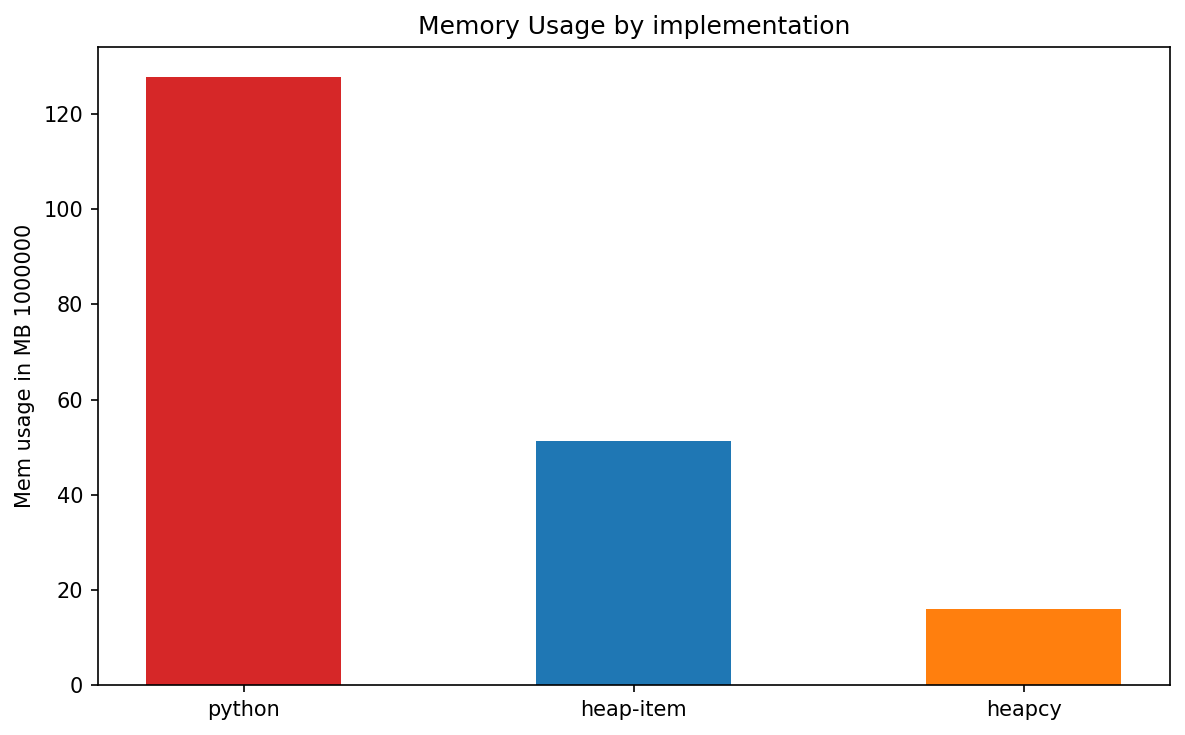
\includegraphics[width=0.8\linewidth]{img/benchmark-1000000.png}
     \caption{Comparative analysis of memory consumption across the three sampling strategies for a batch of $10^6$ items. The \texttt{heapcy} (Custom-heap) implementation demonstrates a $\sim87.47\%$ reduction in memory usage compared to the baseline \texttt{Pure Python} approach. This drastic drop is attributed to the file-offset mechanism (Section \ref{customheap}), which eliminates the overhead of storing string objects in RAM The reduction in memory is not only an efficiency gain it changes the problem class from 'requires a supercomputer' to 'runs on a laptop'.}
     \label{fig:1}
 \end{figure}

\begin{table}[h!tbp]
    \renewcommand{\thetable}{\arabic{table}} % Removes the chapter prefix (e.g., "5.")
    \setcounter{table}{0}                   % Resets the counter to 0
    \centering
    \begin{tabular}{l|c|c|c}
         \toprule
         \#Item & Pure Python &  Heap Item & Heapcy \\
         \midrule
         \rowcolor{lightgray}
         $10^6$ &  127.72 & 51.36 & 16.00\\
         $10^5$ & 12.77 & 5.13 & 1.60\\
         \bottomrule
    \end{tabular}
    \caption{Size occupied in MB for $10^x$  amount of items by each implementation, this tells us how good the optimizations are instead of the old implementation}
    \label{tab:1}
\end{table}
As can be seen the gains have the same rate at any amount of items, so by using 10x the amount of items we will have 10x the amount of memory used.


\subsection{Evaluating Monte Carlo}

\begin{figure}[h!tbp]
\begin{subfigure}[b]{0.32\textwidth}
     \centering
     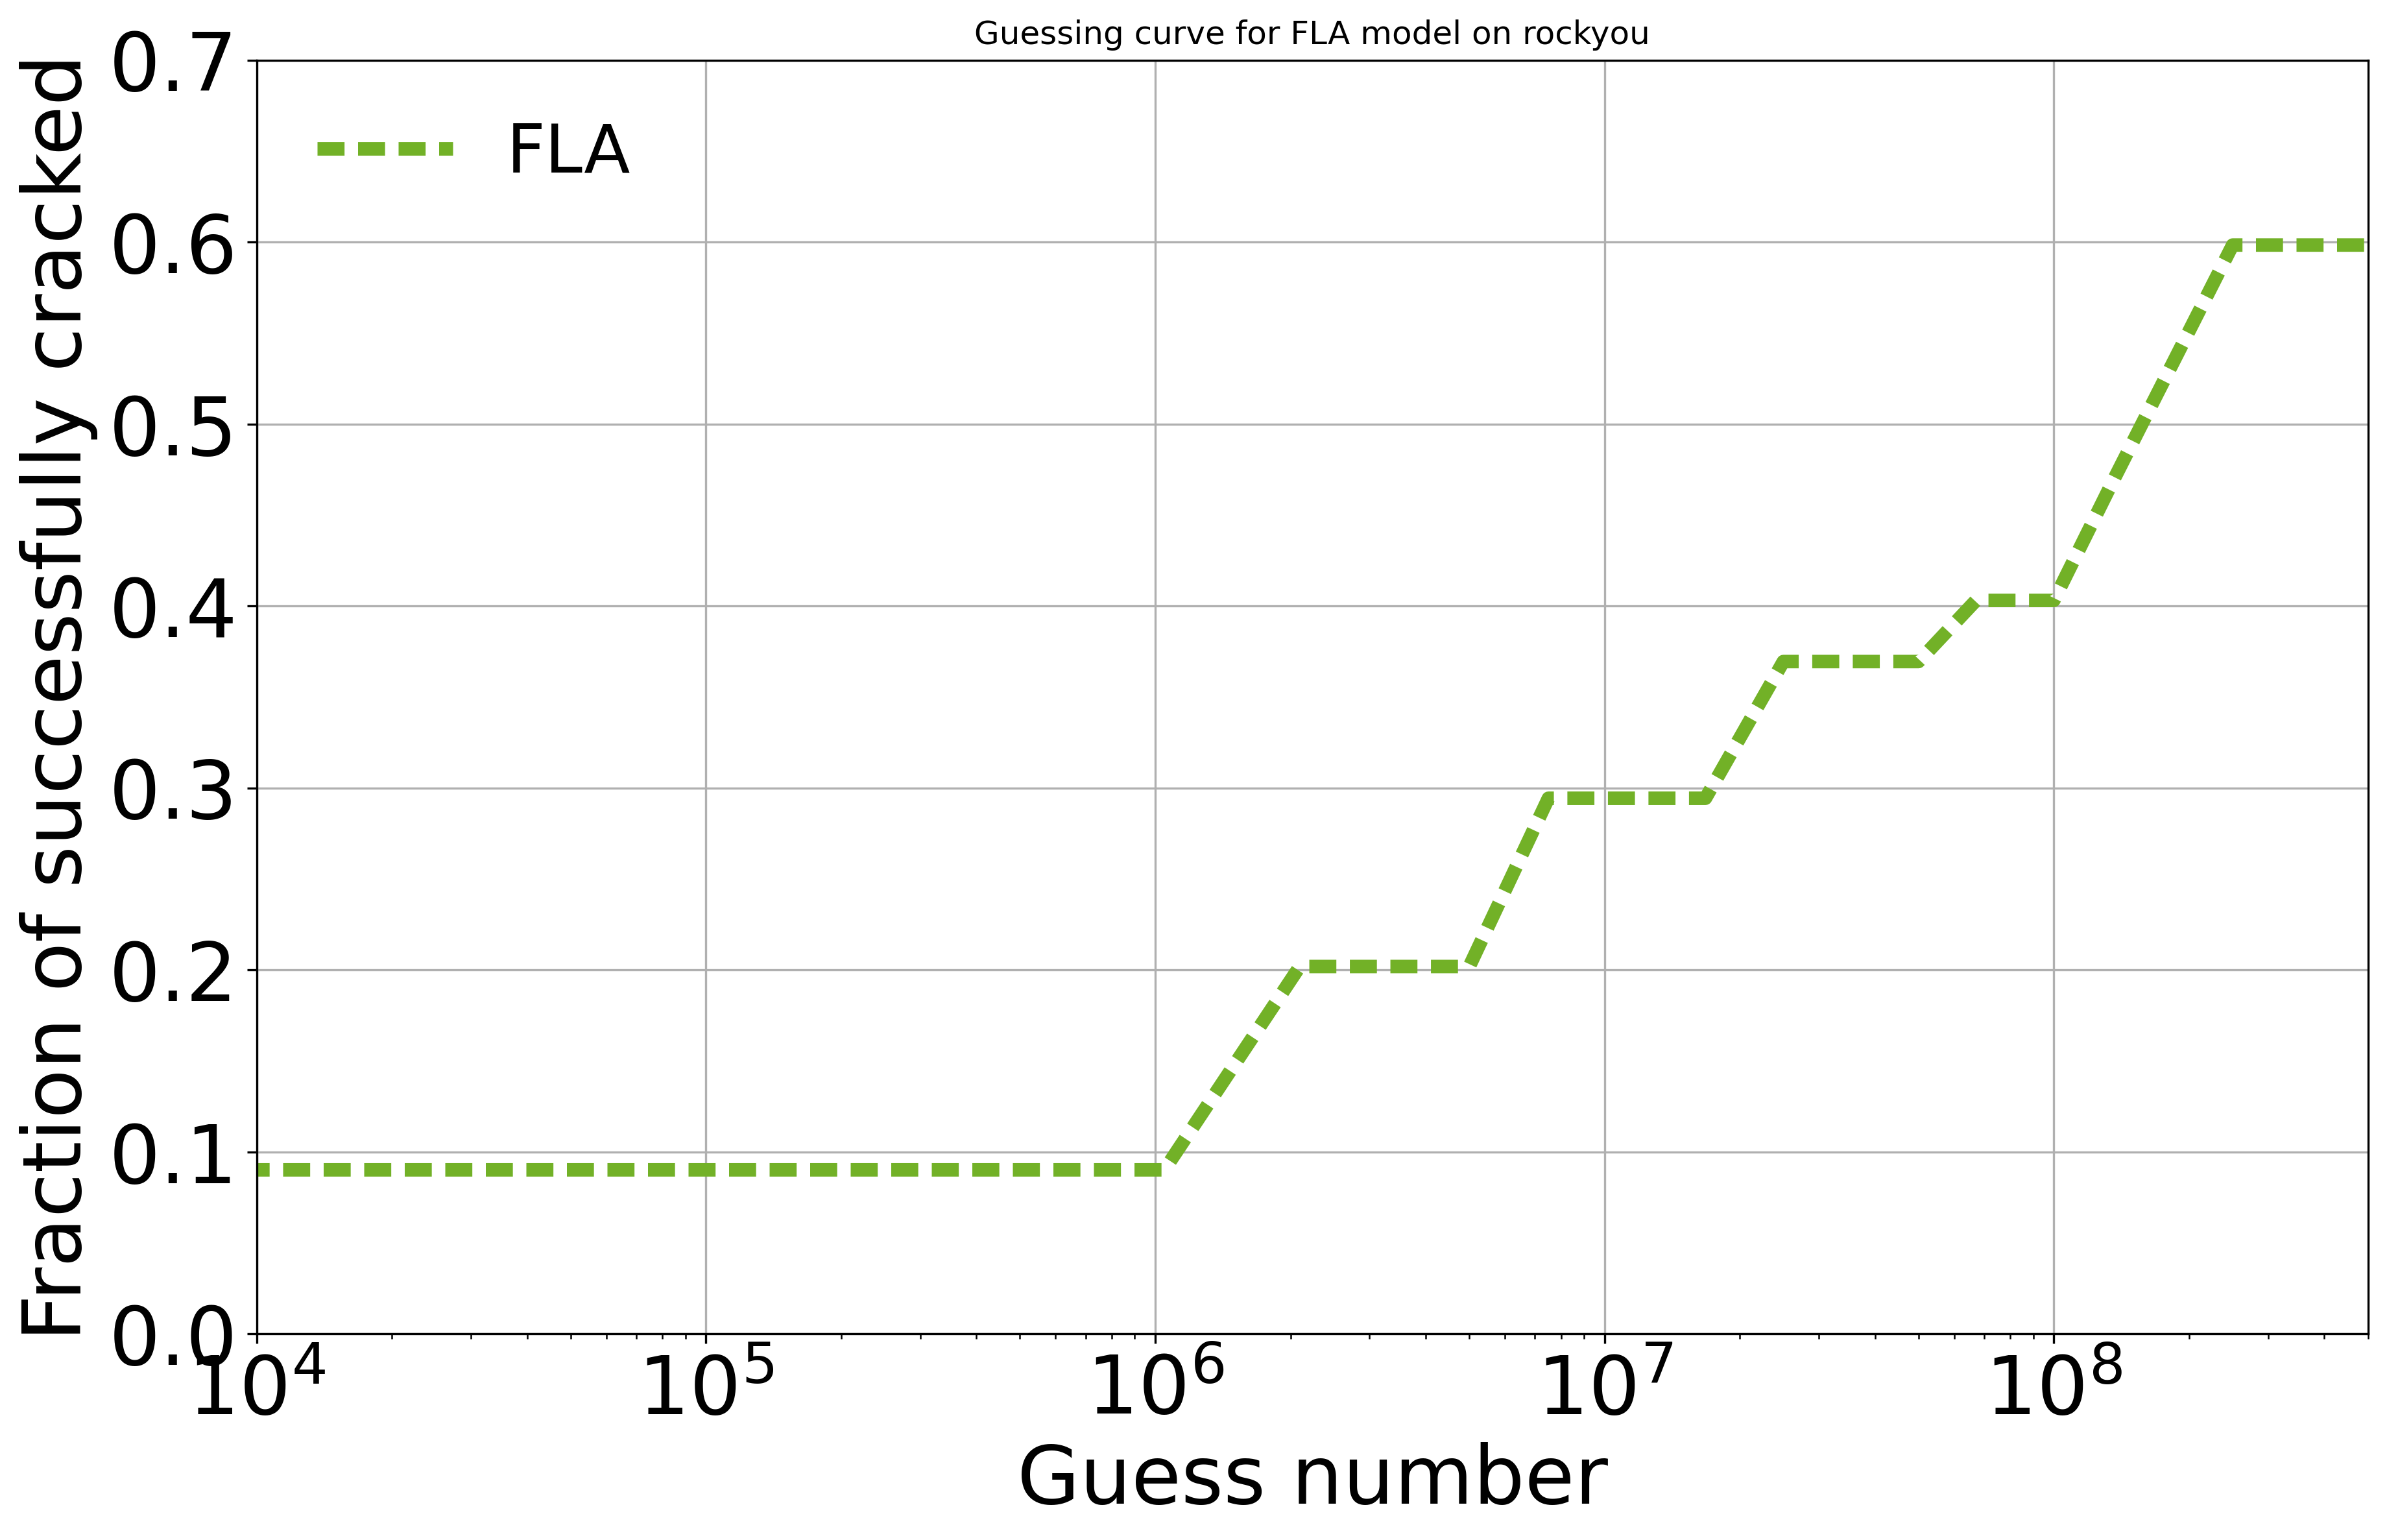
\includegraphics[width=\textwidth]{img/guess_pcg_10.png}
     \caption{Guess \% with a $|\Theta| = 10^1$}
     \label{fig:2a}
 \end{subfigure}
 \hfill
\begin{subfigure}[b]{0.32\textwidth}
     \centering
     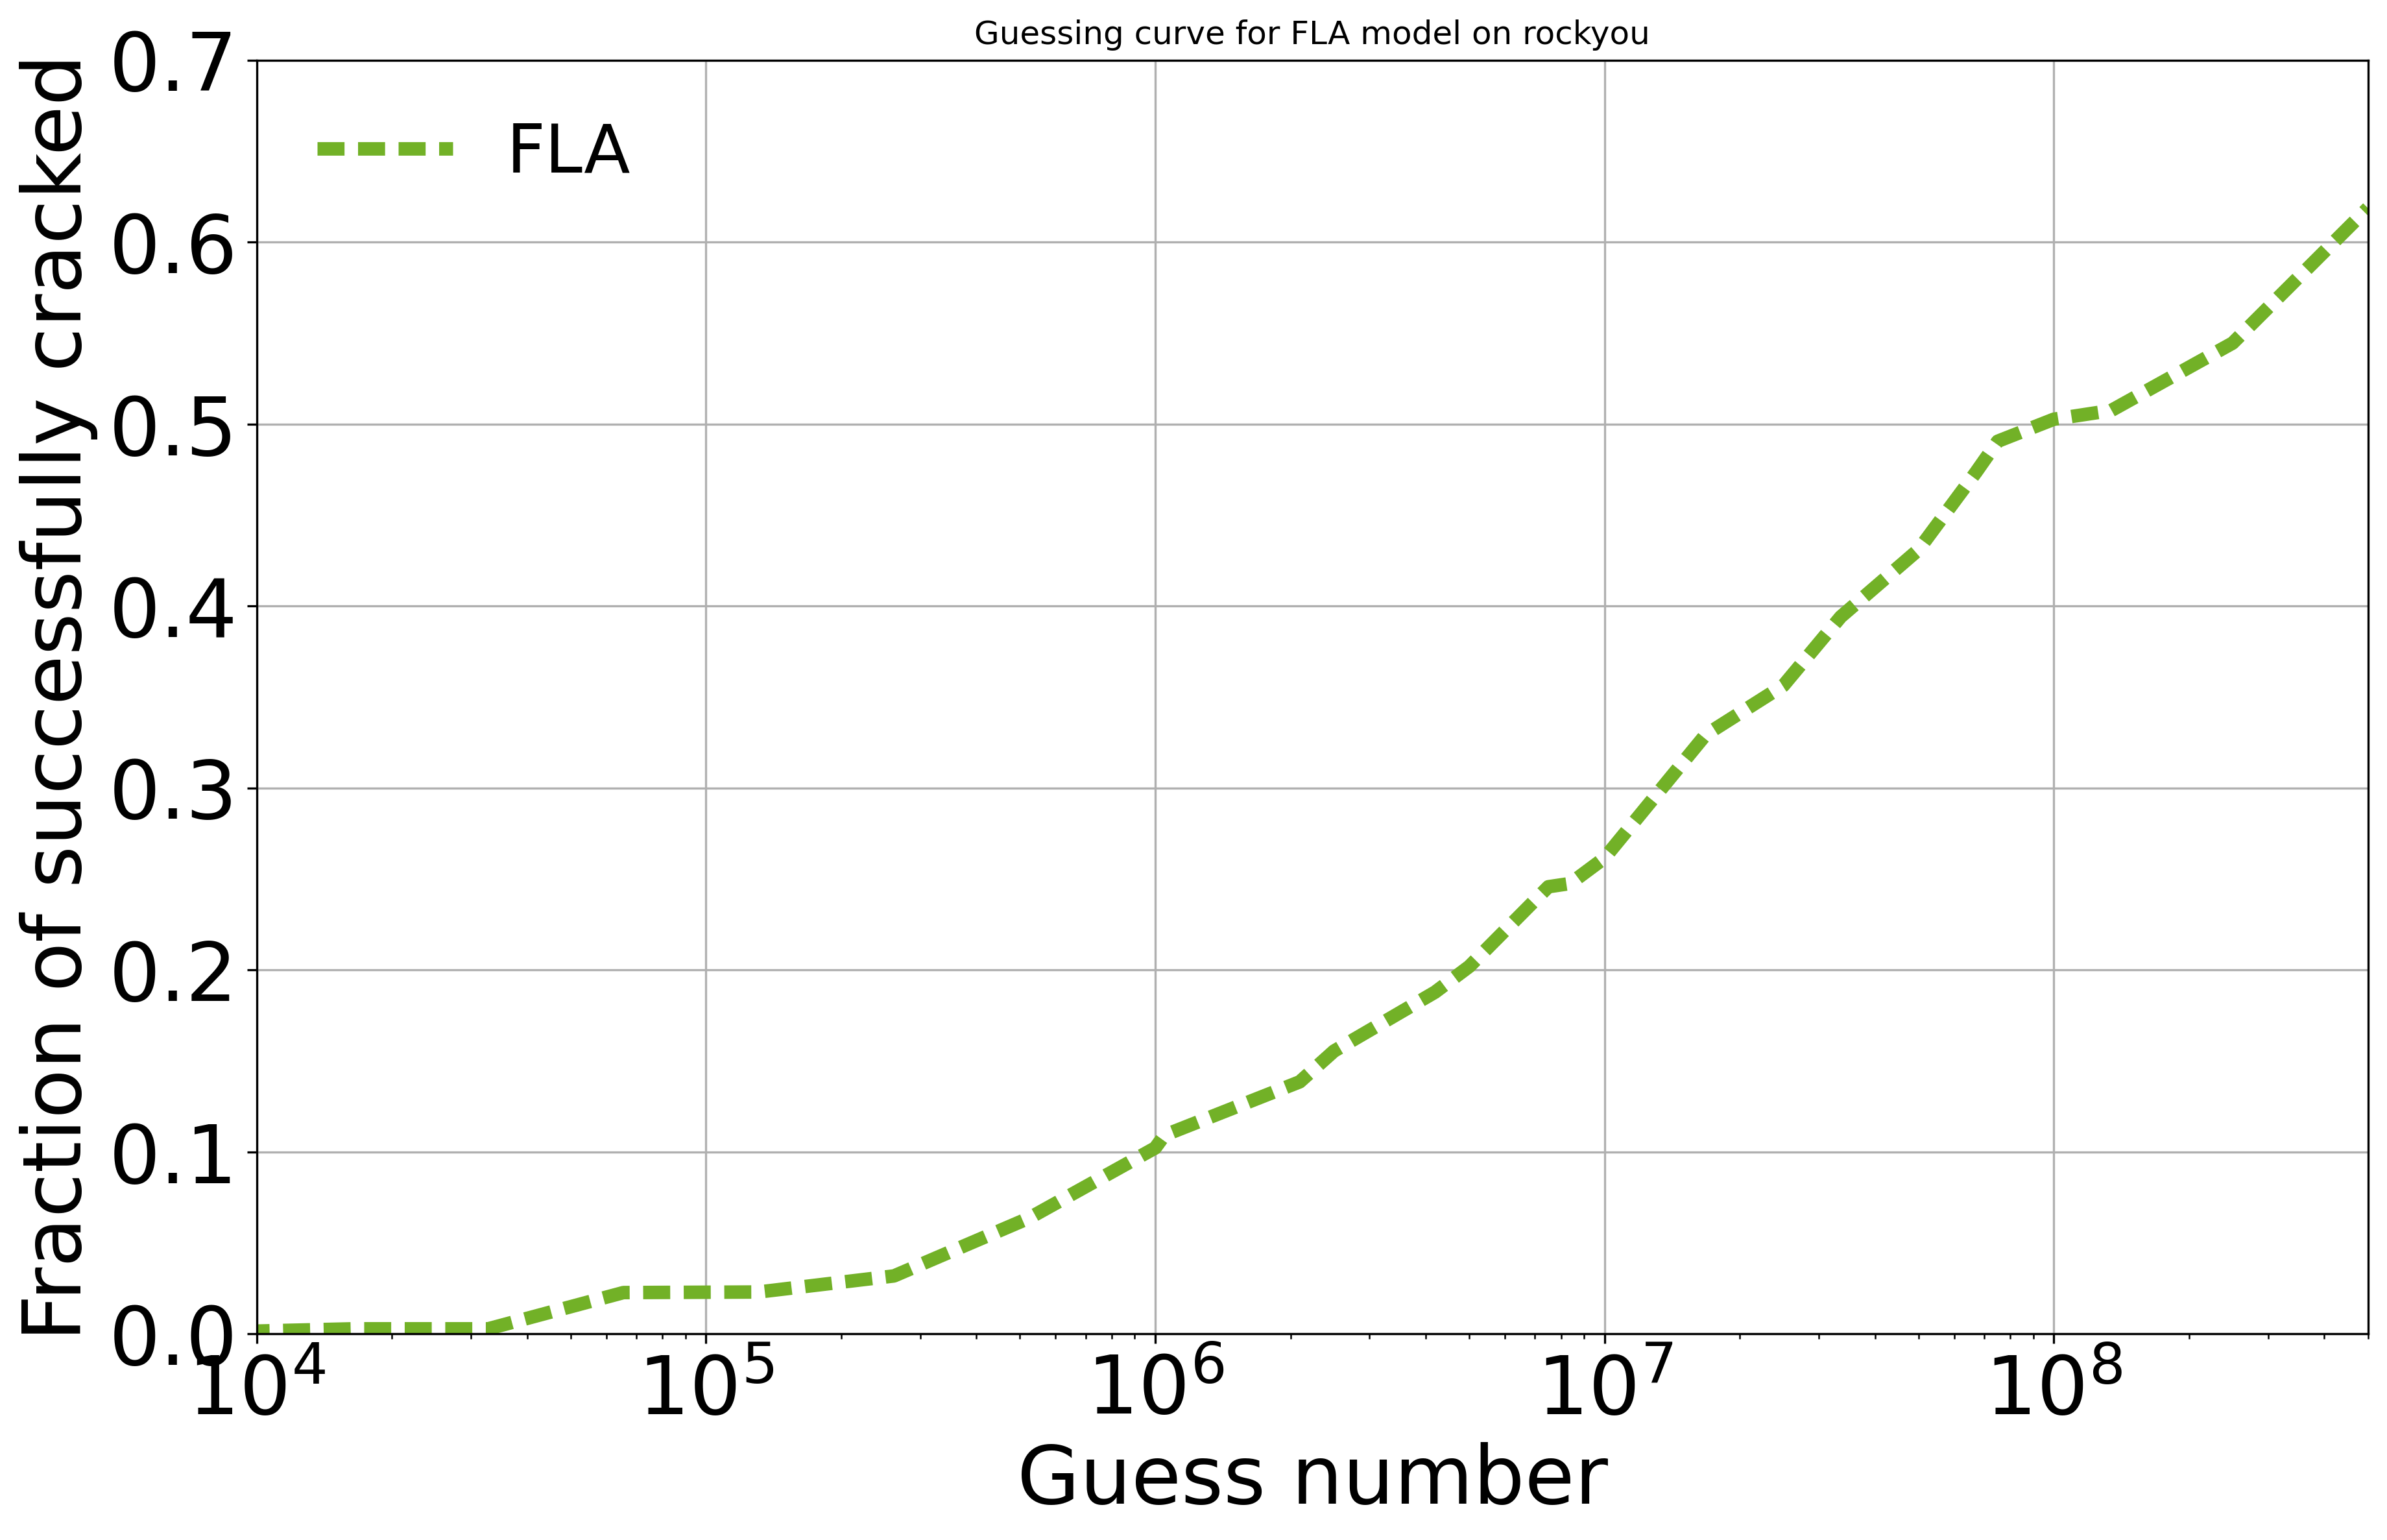
\includegraphics[width=\textwidth]{img/guess_pcg_100.png}
     \caption{Guess \% with a $|\Theta| = 10^2$}
     \label{fig:2b}
 \end{subfigure}
\begin{subfigure}[b]{0.32\textwidth}
     \centering
     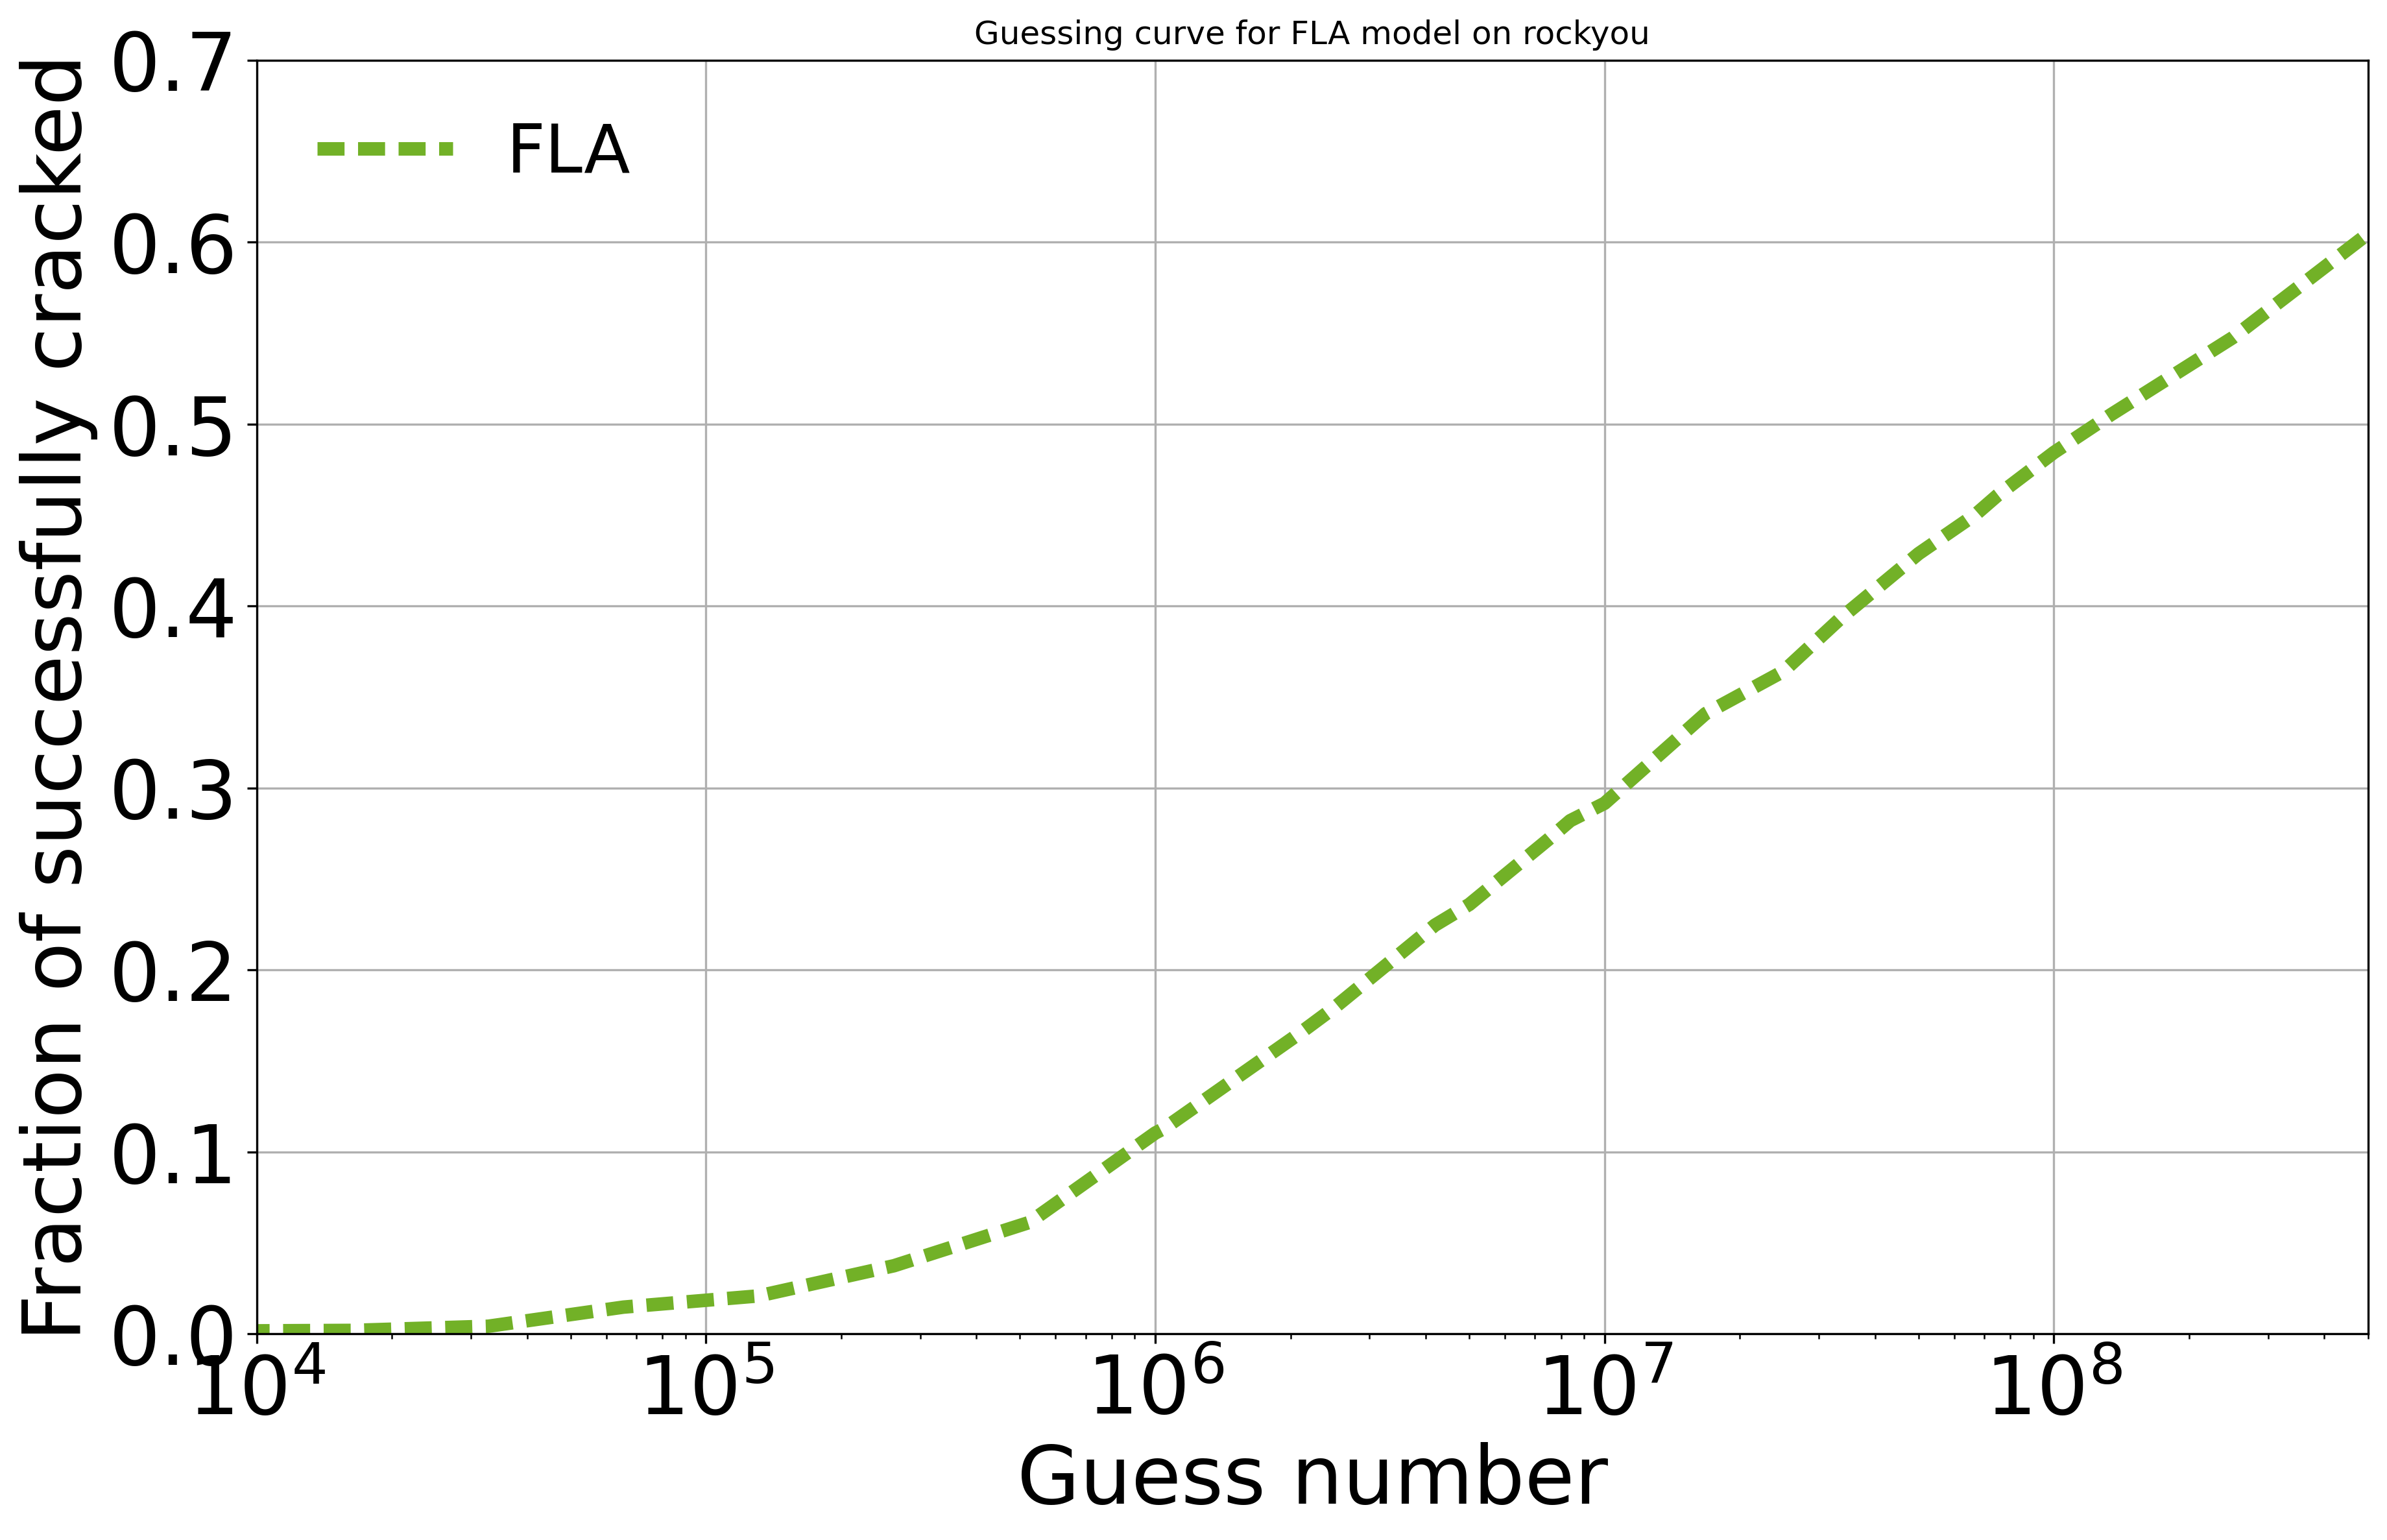
\includegraphics[width=\textwidth]{img/guess_pcg_1000.png}
     \caption{Guess \% with a $|\Theta| = 10^3$}
     \label{fig:2c}
 \end{subfigure}
 
 \vspace{2mm} % Adds vertical space between rows
  \begin{subfigure}[b]{0.32\textwidth}
     \centering
     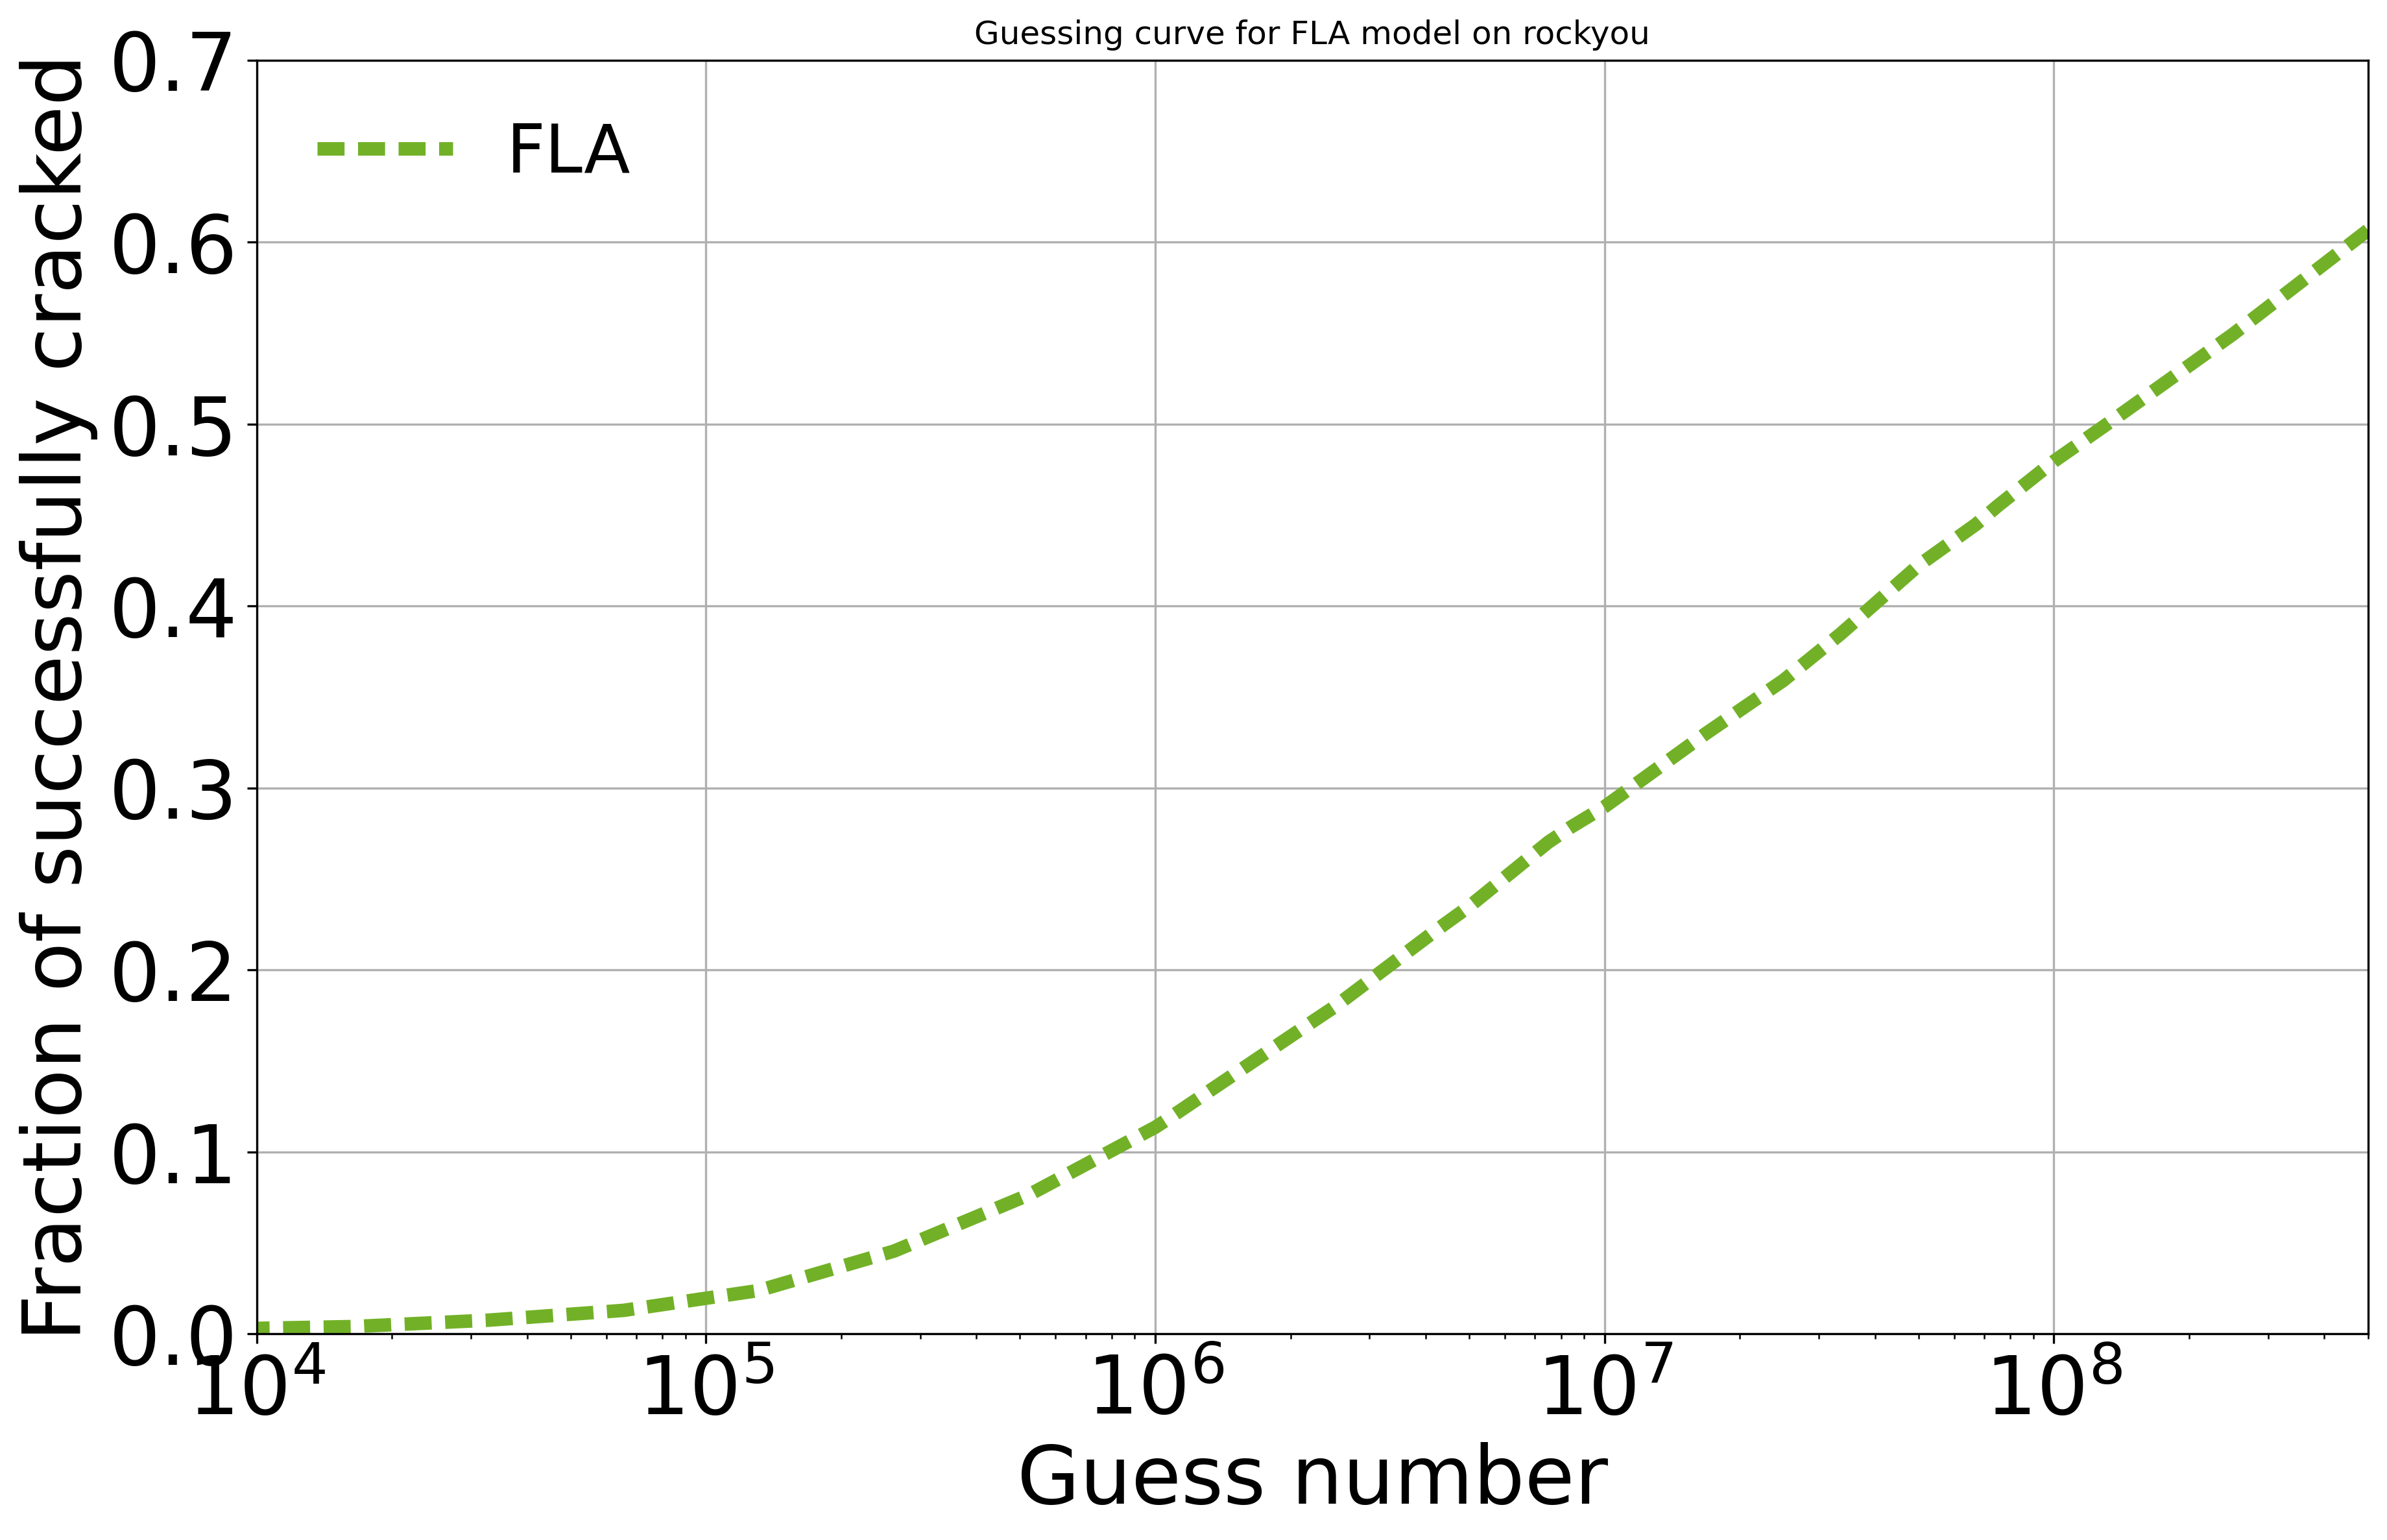
\includegraphics[width=\textwidth]{img/guess_pcg_10000.png}
     \caption{Guess \% with a $|\Theta| = 10^4$}
     \label{fig:2d}
 \end{subfigure}
 \hfill
\begin{subfigure}[b]{0.32\textwidth}
     \centering
     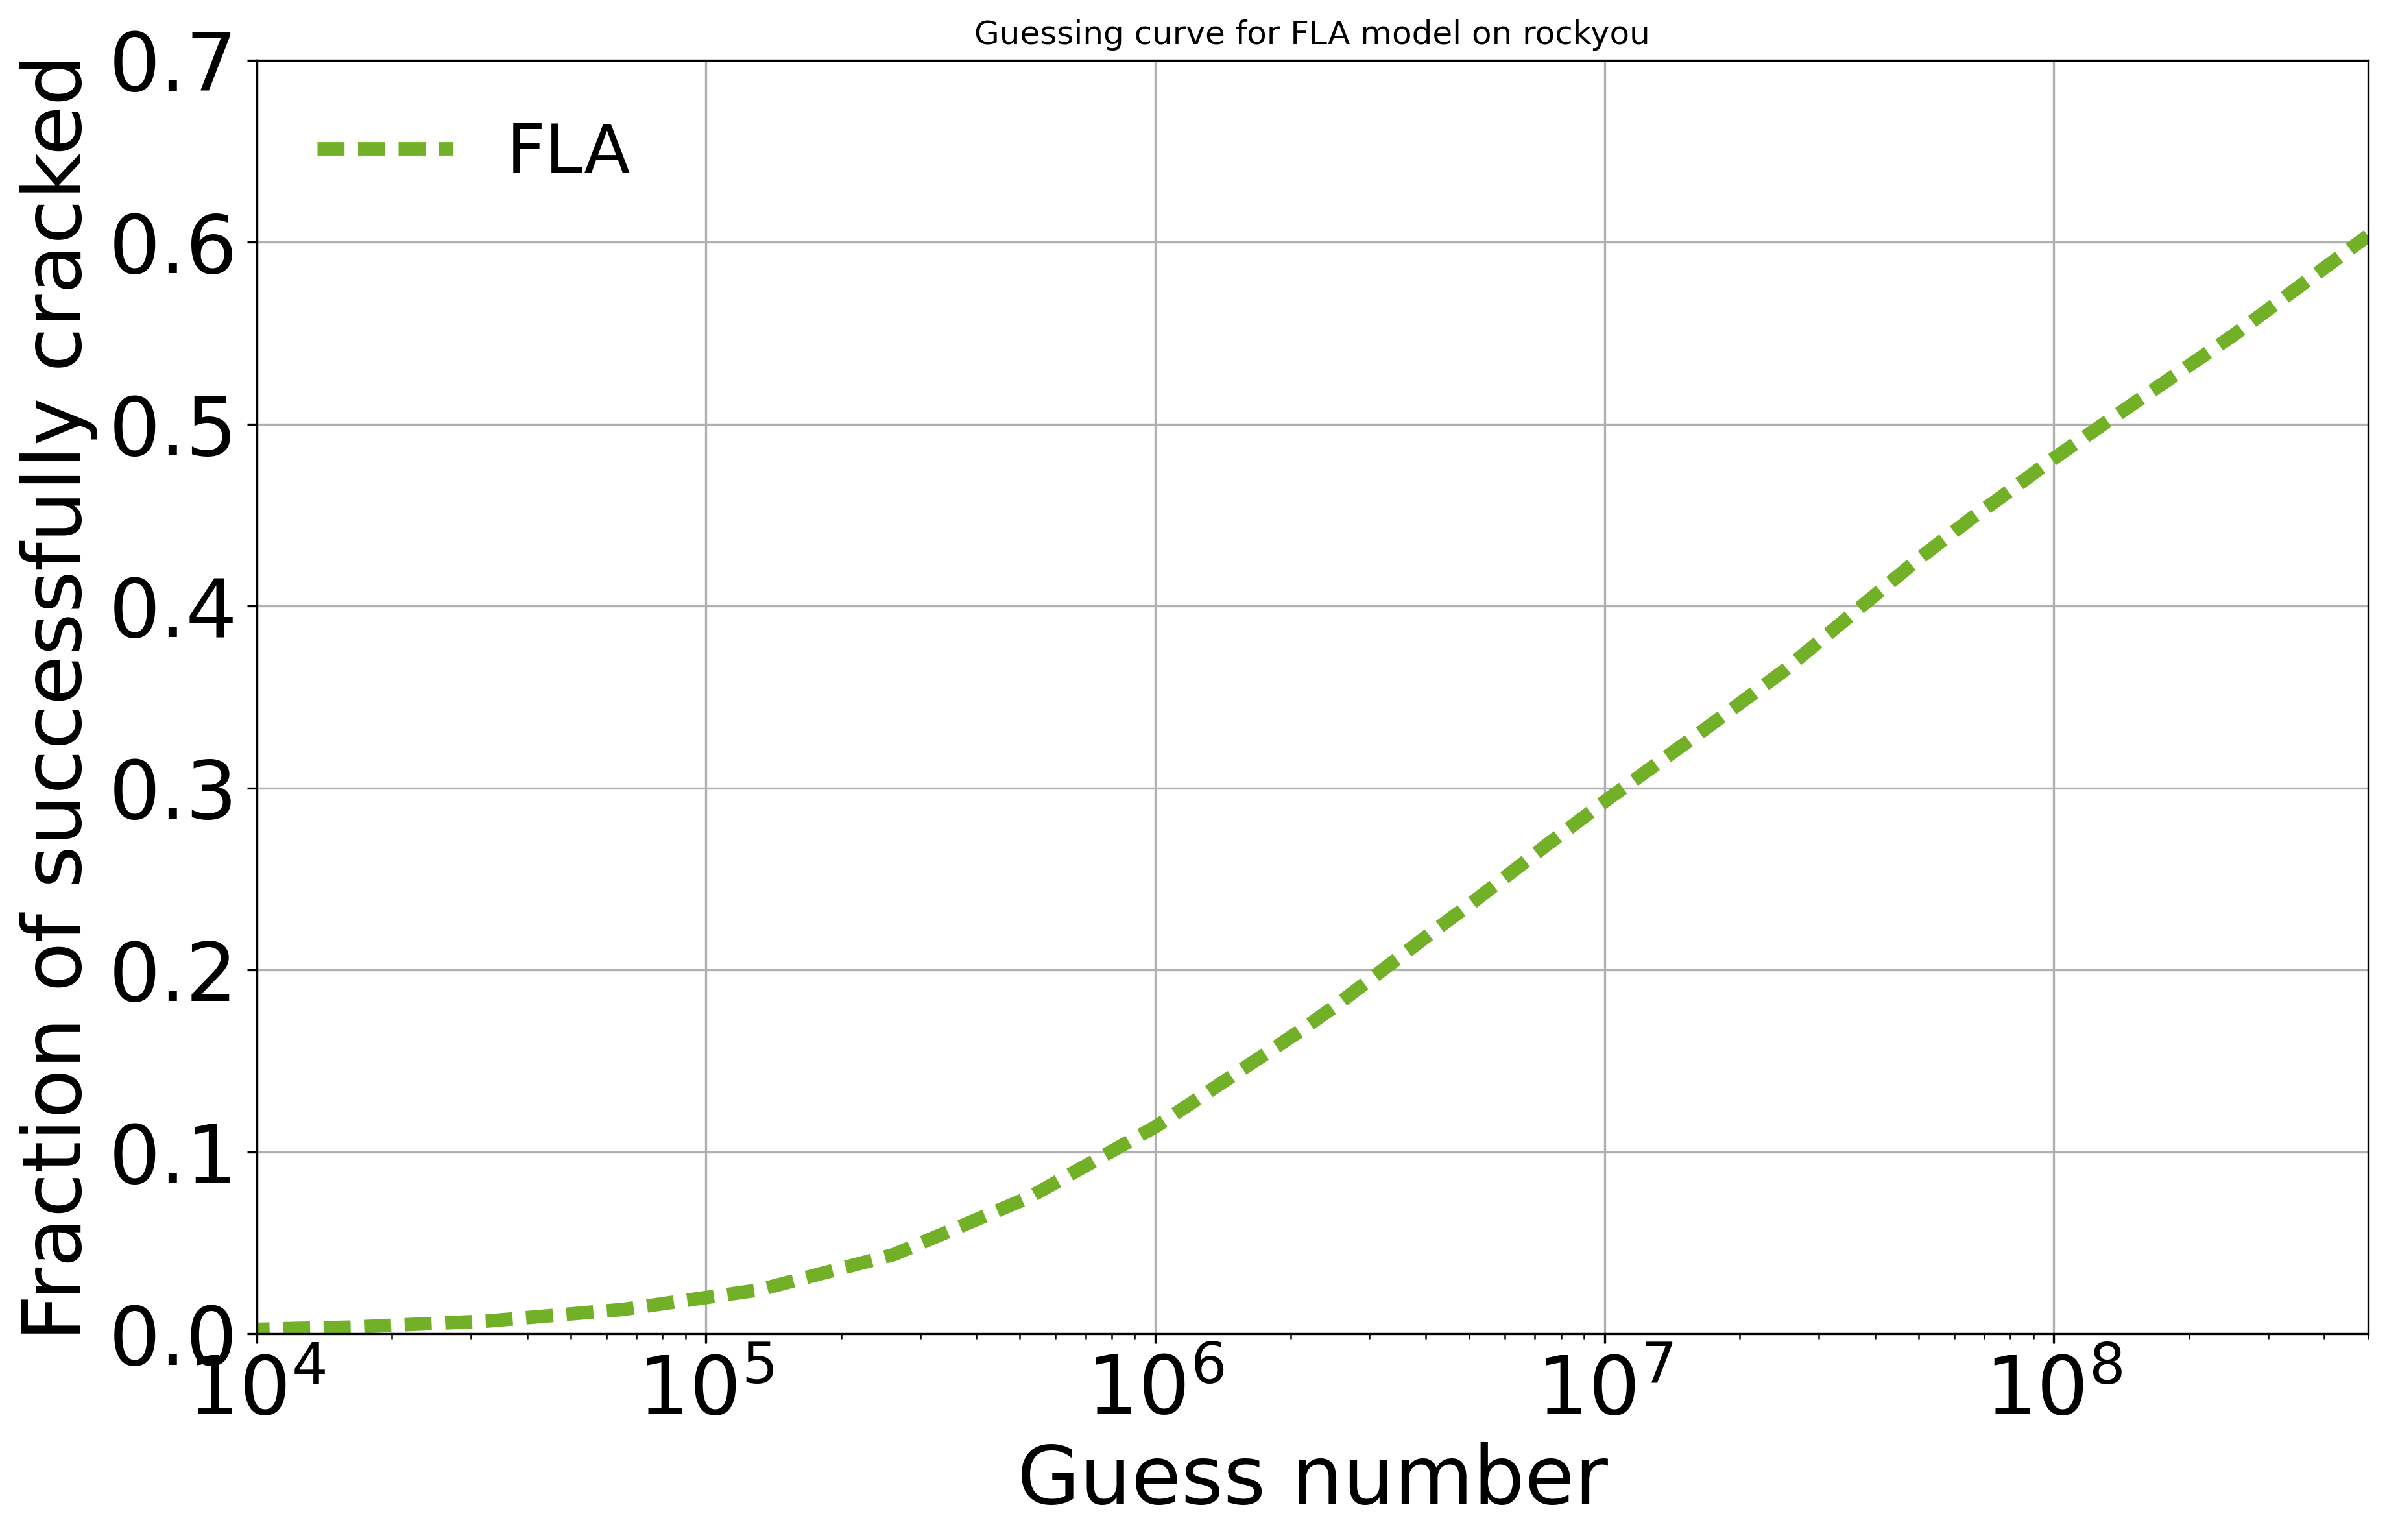
\includegraphics[width=\textwidth]{img/guess_pcg_100000.png}
     \caption{Guess \% with a $|\Theta| = 10^5$}
     \label{fig:2e}
 \end{subfigure}
 \hfill
 \begin{subfigure}[b]{0.32\textwidth}
     \centering
     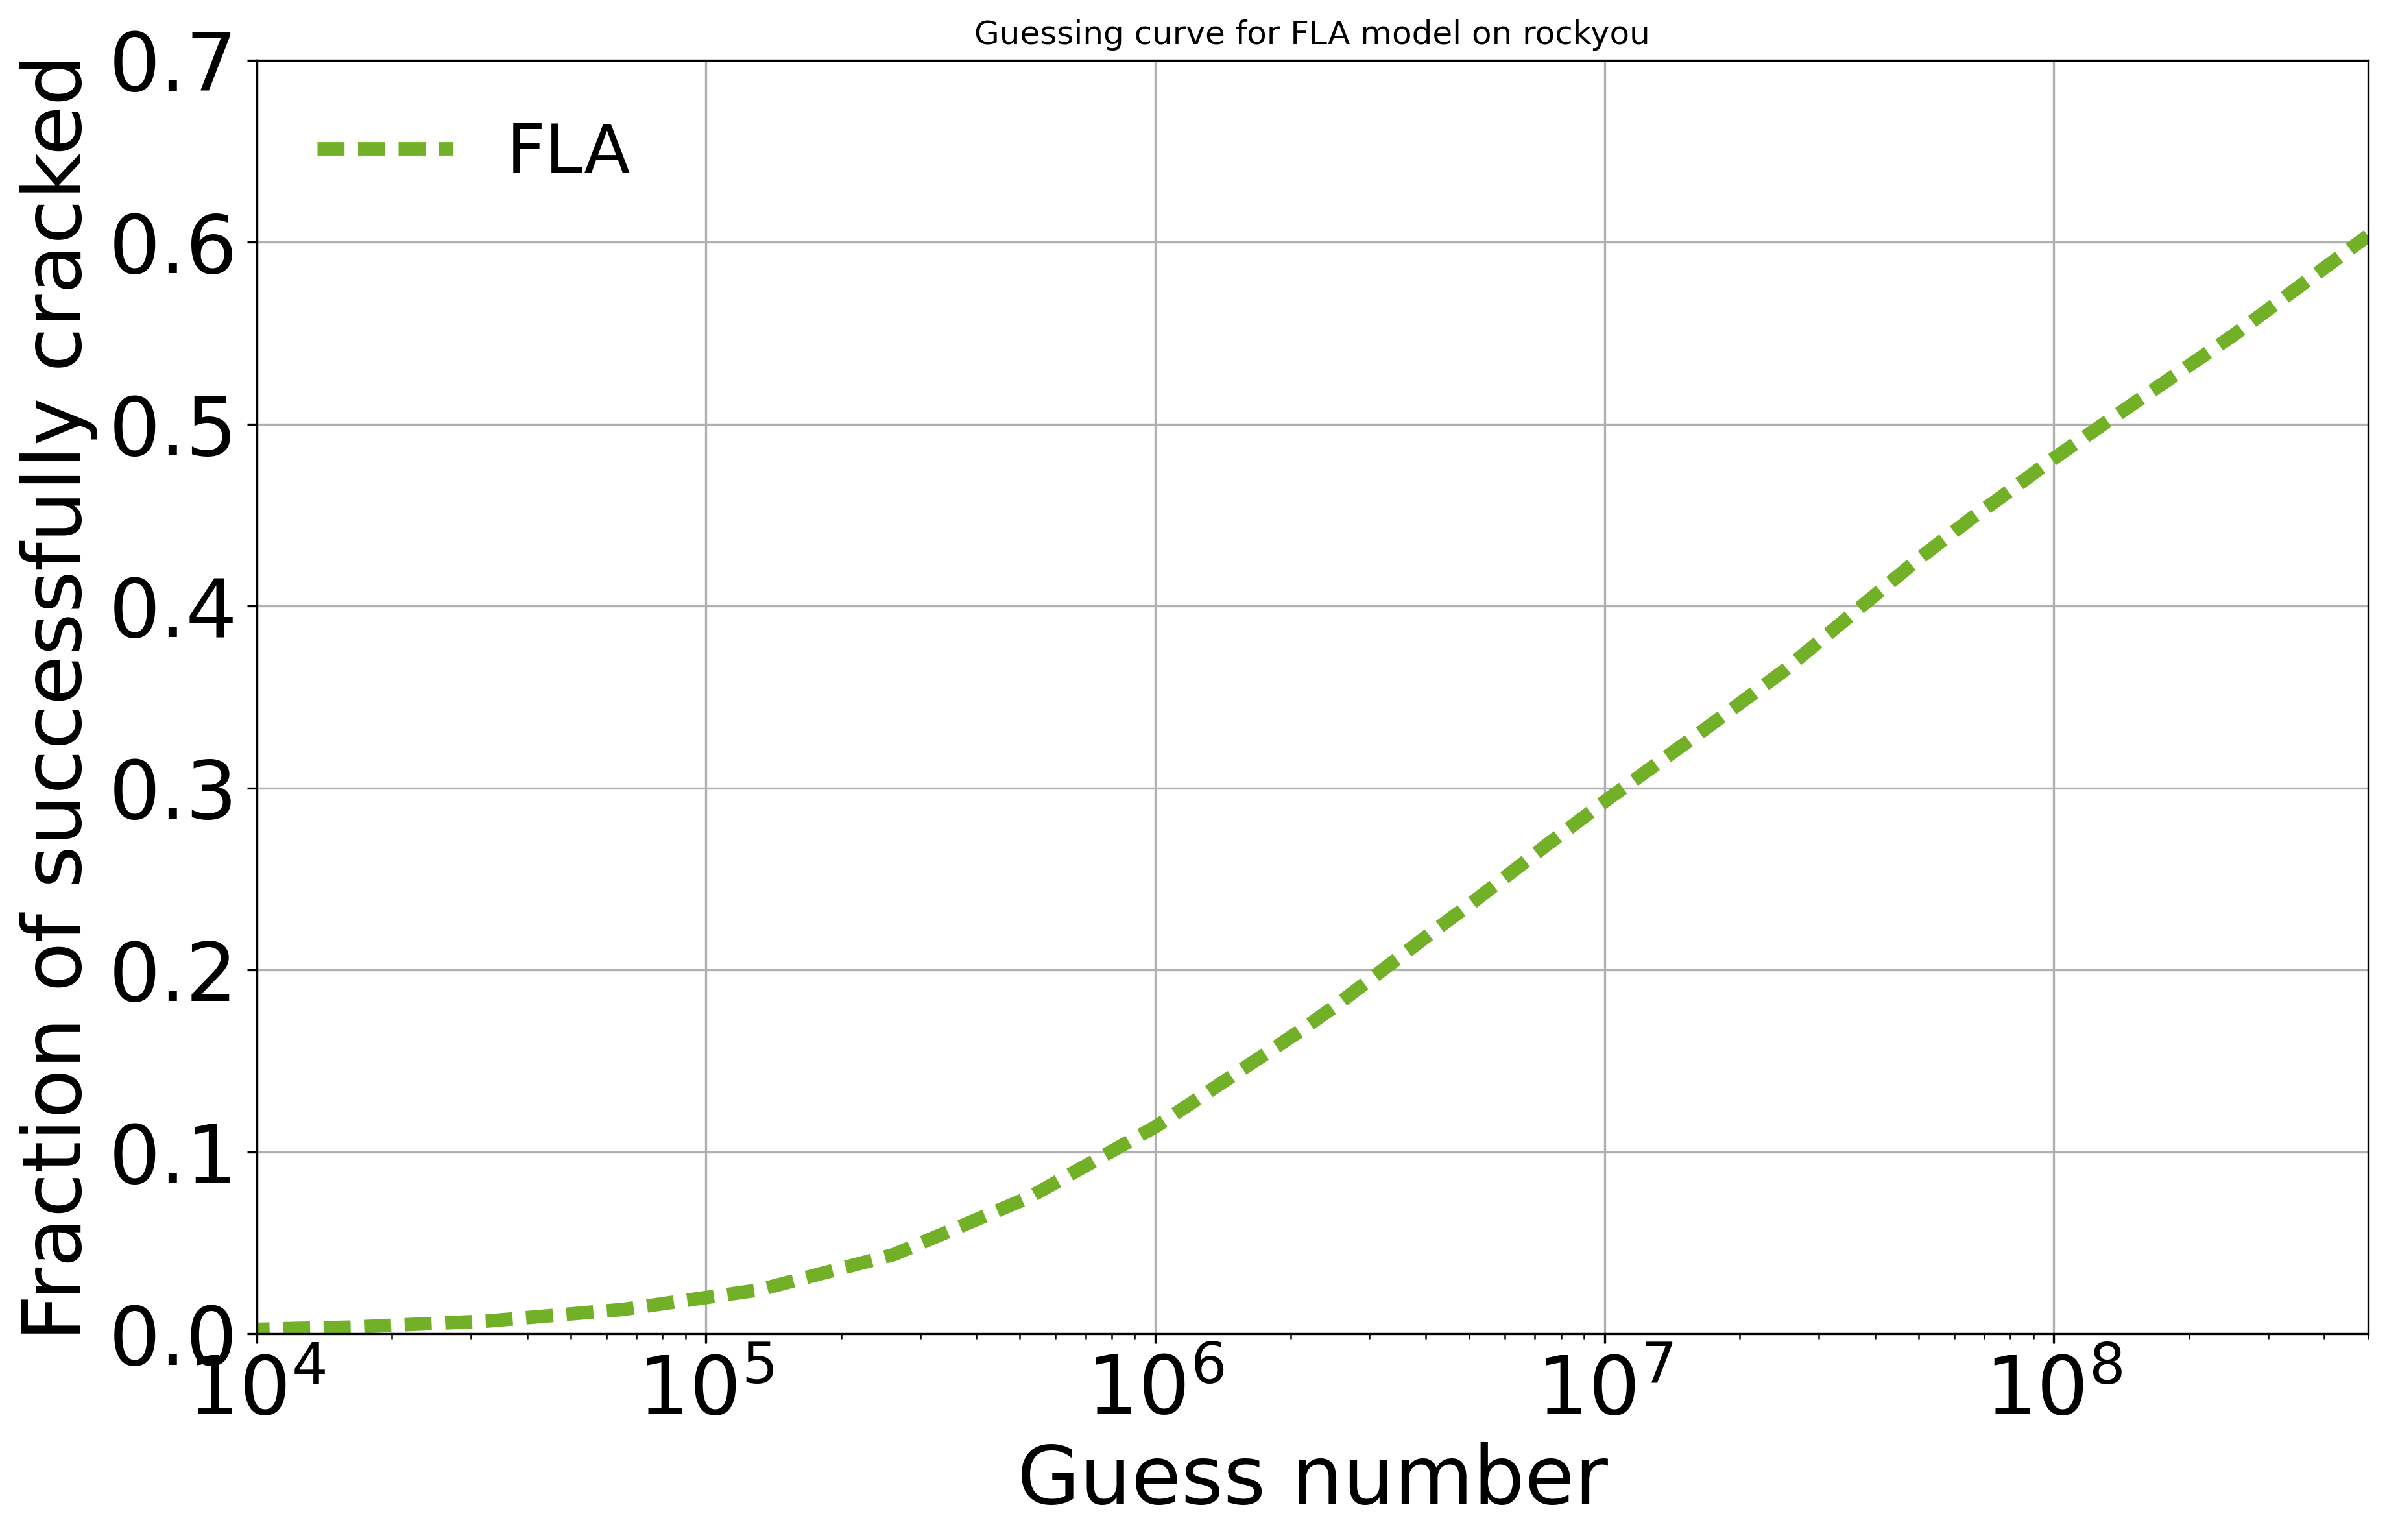
\includegraphics[width=\textwidth]{img/guess_pcg_100000.png}
     \caption{Guess \% with a $|\Theta| = 10^6$}
     \label{fig:2f}
 \end{subfigure}
\end{figure}
\begin{figure}[h!]
    \centering
       \renewcommand{\thefigure}{\arabic{figure}} % Removes the chapter prefix (e.g., "5.")
    \setcounter{figure}{1}      
    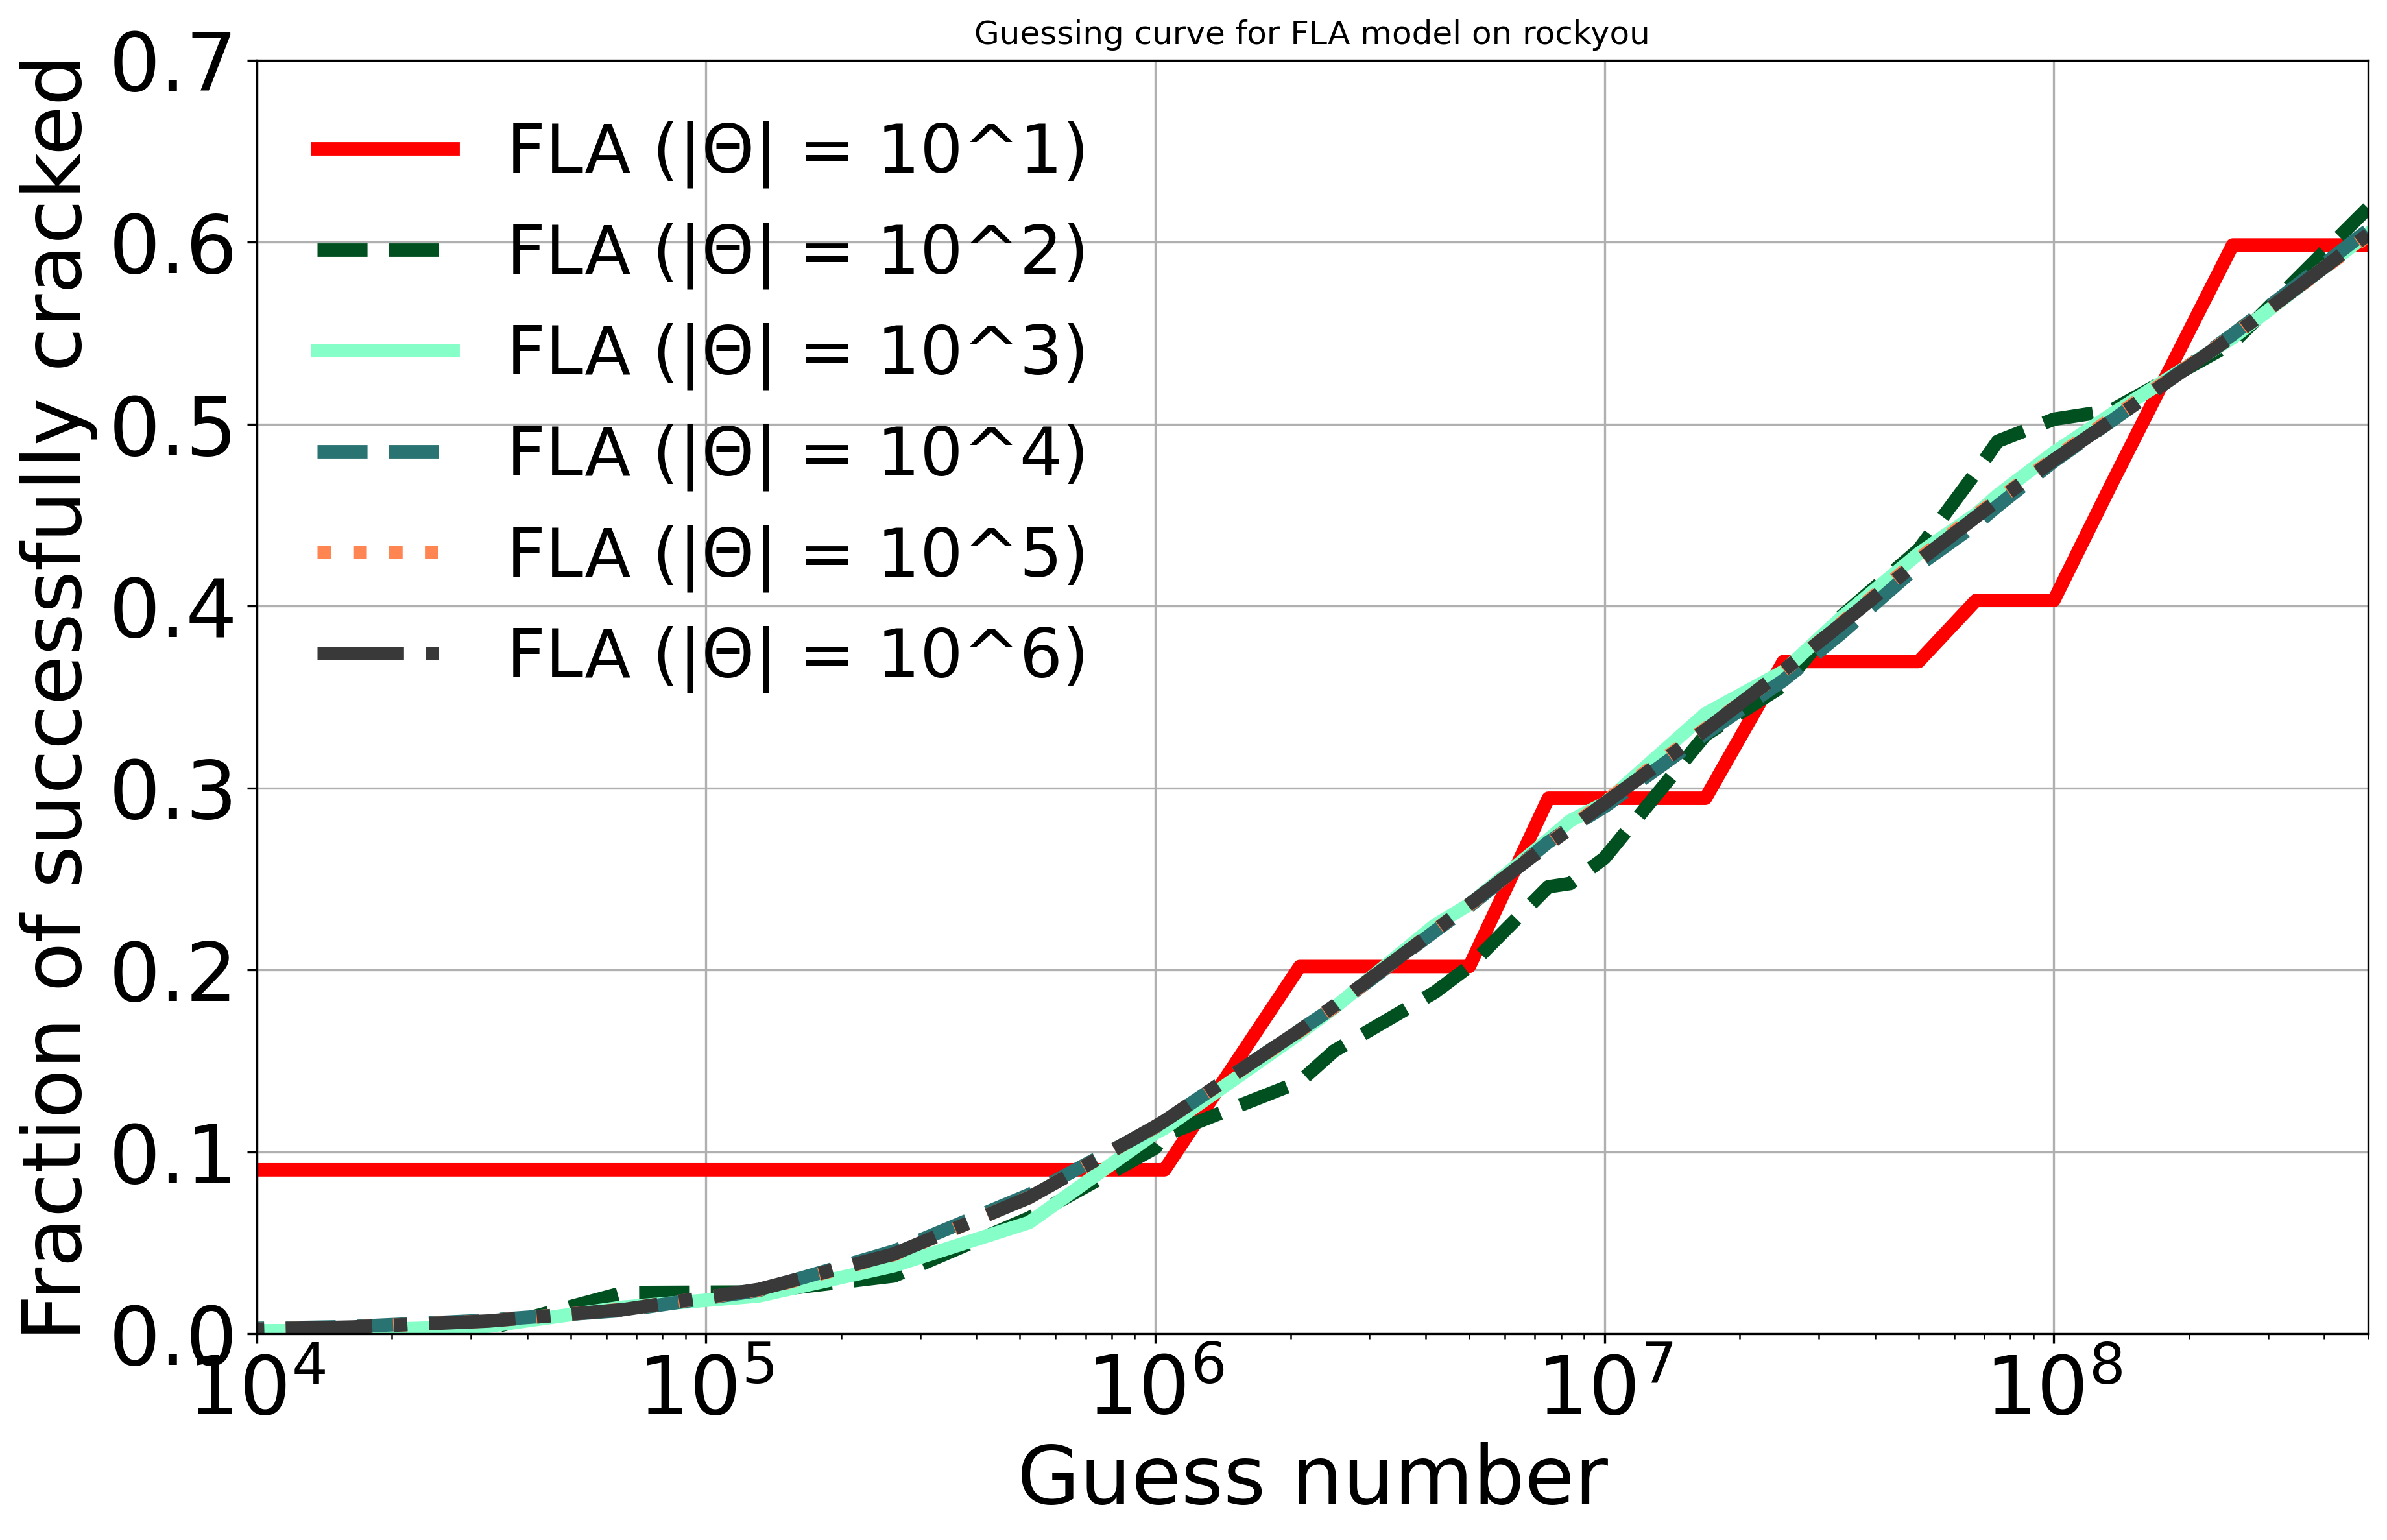
\includegraphics[width=0.85\linewidth]{img/guess_pcg_combined.png}
    \caption{Convergence of the Monte Carlo rank estimation as the sample size $|\theta|$ increases.
Subfigures $(a)$ through $(d)$illustrate that at lower sample sizes $(10^1,10^2,10^3)$, the estimation exhibits high variance (noise). As $|\Theta|$ approaches $10^5$and $10^6$ (f), the curve stabilizes confirming that sample sizes large enough produce deterministic like accuracy.}
    \label{fig:3}
\end{figure}
\FloatBarrier

\begin{table}[htbp]
\renewcommand{\thetable}{\arabic{table}} % Removes the chapter prefix (e.g., "5.")
\setcounter{table}{1}                   % Resets the counter to 1
\centering
\setlength{\tabcolsep}{3pt}
\begin{tabular}{l|r|r|r|r|r|r|r}
\toprule
Guess \# & Rate $10^1$ & Rate $10^2$ & Rate $10^3$ & Rate $10^4$ & Rate $10^5$ & Rate $10^6$ & MAYA \% \\
\midrule
% --- FIRST COLUMN IS NOW IN SCIENTIFIC NOTATION ---
\rowcolor{lightgray}
$1.0 \cdot 10^6$ & $9.01\%$ & $10.22\%$ & $11.03\%$ & $11.35\%$ & $11.37\%$ & $11.40\%$ & $11.40\%$ \\
$2.5 \cdot 10^6$ & $20.19\%$ & $15.54\%$ & $17.91\%$ & $17.95\%$ & $17.97\%$ & $18.02\%$ & $18.04\%$ \\
\rowcolor{lightgray}
$5.0 \cdot 10^6$ & $20.19\%$ &$20.19\%$ & $23.60\%$ & $23.49\%$ & $23.57\%$ & $23.61\%$ & $23.66\%$ \\
$7.5 \cdot 10^6$ & $29.43\%$ &$24.57\%$ & $27.17\%$ & $27.02\%$ & $26.94\%$ & $26.90\%$ & $26.94\%$ \\
\rowcolor{lightgray}
$1.0 \cdot 10^7$ & $29.43\%$ &$26.15.\%$ & $29.15\%$ & $28.97\%$ & $29.25\%$ & $29.16\%$ & $29.20\%$ \\

$2.5 \cdot 10^7$ & $36.95\%$ &$35.63\%$ & $36.41\%$ & $35.91\%$ & $36.42\%$ & $36.45\%$ & $36.48\%$ \\
\rowcolor{lightgray}
$5.0 \cdot 10^7$ & $36.95\%$ &$43.09\%$ & $42.88\%$ & $42.23\%$ & $42.59\%$ & $42.47\%$ & $42.49\%$ \\
$7.5 \cdot 10^7$ &$40.31\%$ & $49.05\%$ & $46.09\%$ & $45.50\%$ & $45.84\%$ & $45.80\%$ & $45.82\%$ \\
\rowcolor{lightgray}
$1.0 \cdot10^8$ & $40.31\%$ &$50.26\%$ & $48.43\%$ & $47.95\%$ & $48.11\%$ & $48.02\%$ & $48.04\%$ \\
$2.5 \cdot 10^8$ & $59.84\%$ &$54.45\%$ & $54.74\%$ & $54.92\%$ & $54.85\%$ & $54.83\%$ & $54.85\%$ \\
\rowcolor{lightgray}
$5.0 \cdot 10^8$ & $59.84\%$ &$61.87\%$ & $60.45\%$ & $60.65\%$ & $60.35\%$ & $60.42\%$ & $60.47\%$ \\
 \bottomrule
\end{tabular}
\caption{Stability of the Guessing Percentage (G(x)) across varying Monte Carlo sample
sizes. The data indicates that even at low samples $10^4$ the results are close enough to
the deterministic ones.}
\label{tab:2}
\end{table}

\chapter{Conclusion}
\label{chap:7}
In Conclusion we managed to optimize the sampling of FLA, added montecarlo to MAYA and we proved with results how the montecarlo estimation is very good at estimating the evaluation.
We went beyond FLAs original paper by proving the result up to $5.0 \cdot 10^8$ this may imply that we do not need to the evaluation deterministic enumeration, by using enumeration, instead we can use montecarlo to see how good a model really is.
Being able to extend Monte Carlo sampling to $|\Theta| = 5\cdot10^8$ is 
important, since the accuracy of it is entirely dependent on the size of $|\Theta|$ 
The larger the sample size the smaller the variance in the tail of the distribution(Low probability passwords), which is where many
real passwords reside. Our optimizations therefore enable a  better evaluation of password-guessing models without requiring 
enormous amounts of memory usage.
In future works we should expand this method to every model implemented inside of MAYA, and try montecarlo for even larger numbers, since the new optimization allows us to enumerate up to even bigger numbers without incurring into big performance issues.
We should as well optimize the caching part \ref{algo:gen_sorted}, since for now it is all sequential and takes a considerable amount of time $\sim 4hr$ for RockYou test-dataset $\sim 4.0*10^6$ passwords.
We could also improve the heapcy implementation to have a dynamic memory instead of the current implementation.
\chapter{Appendix}
\appendix
\section{UML}
\label{uml}
\begin{figure}[h!]
    \centering
    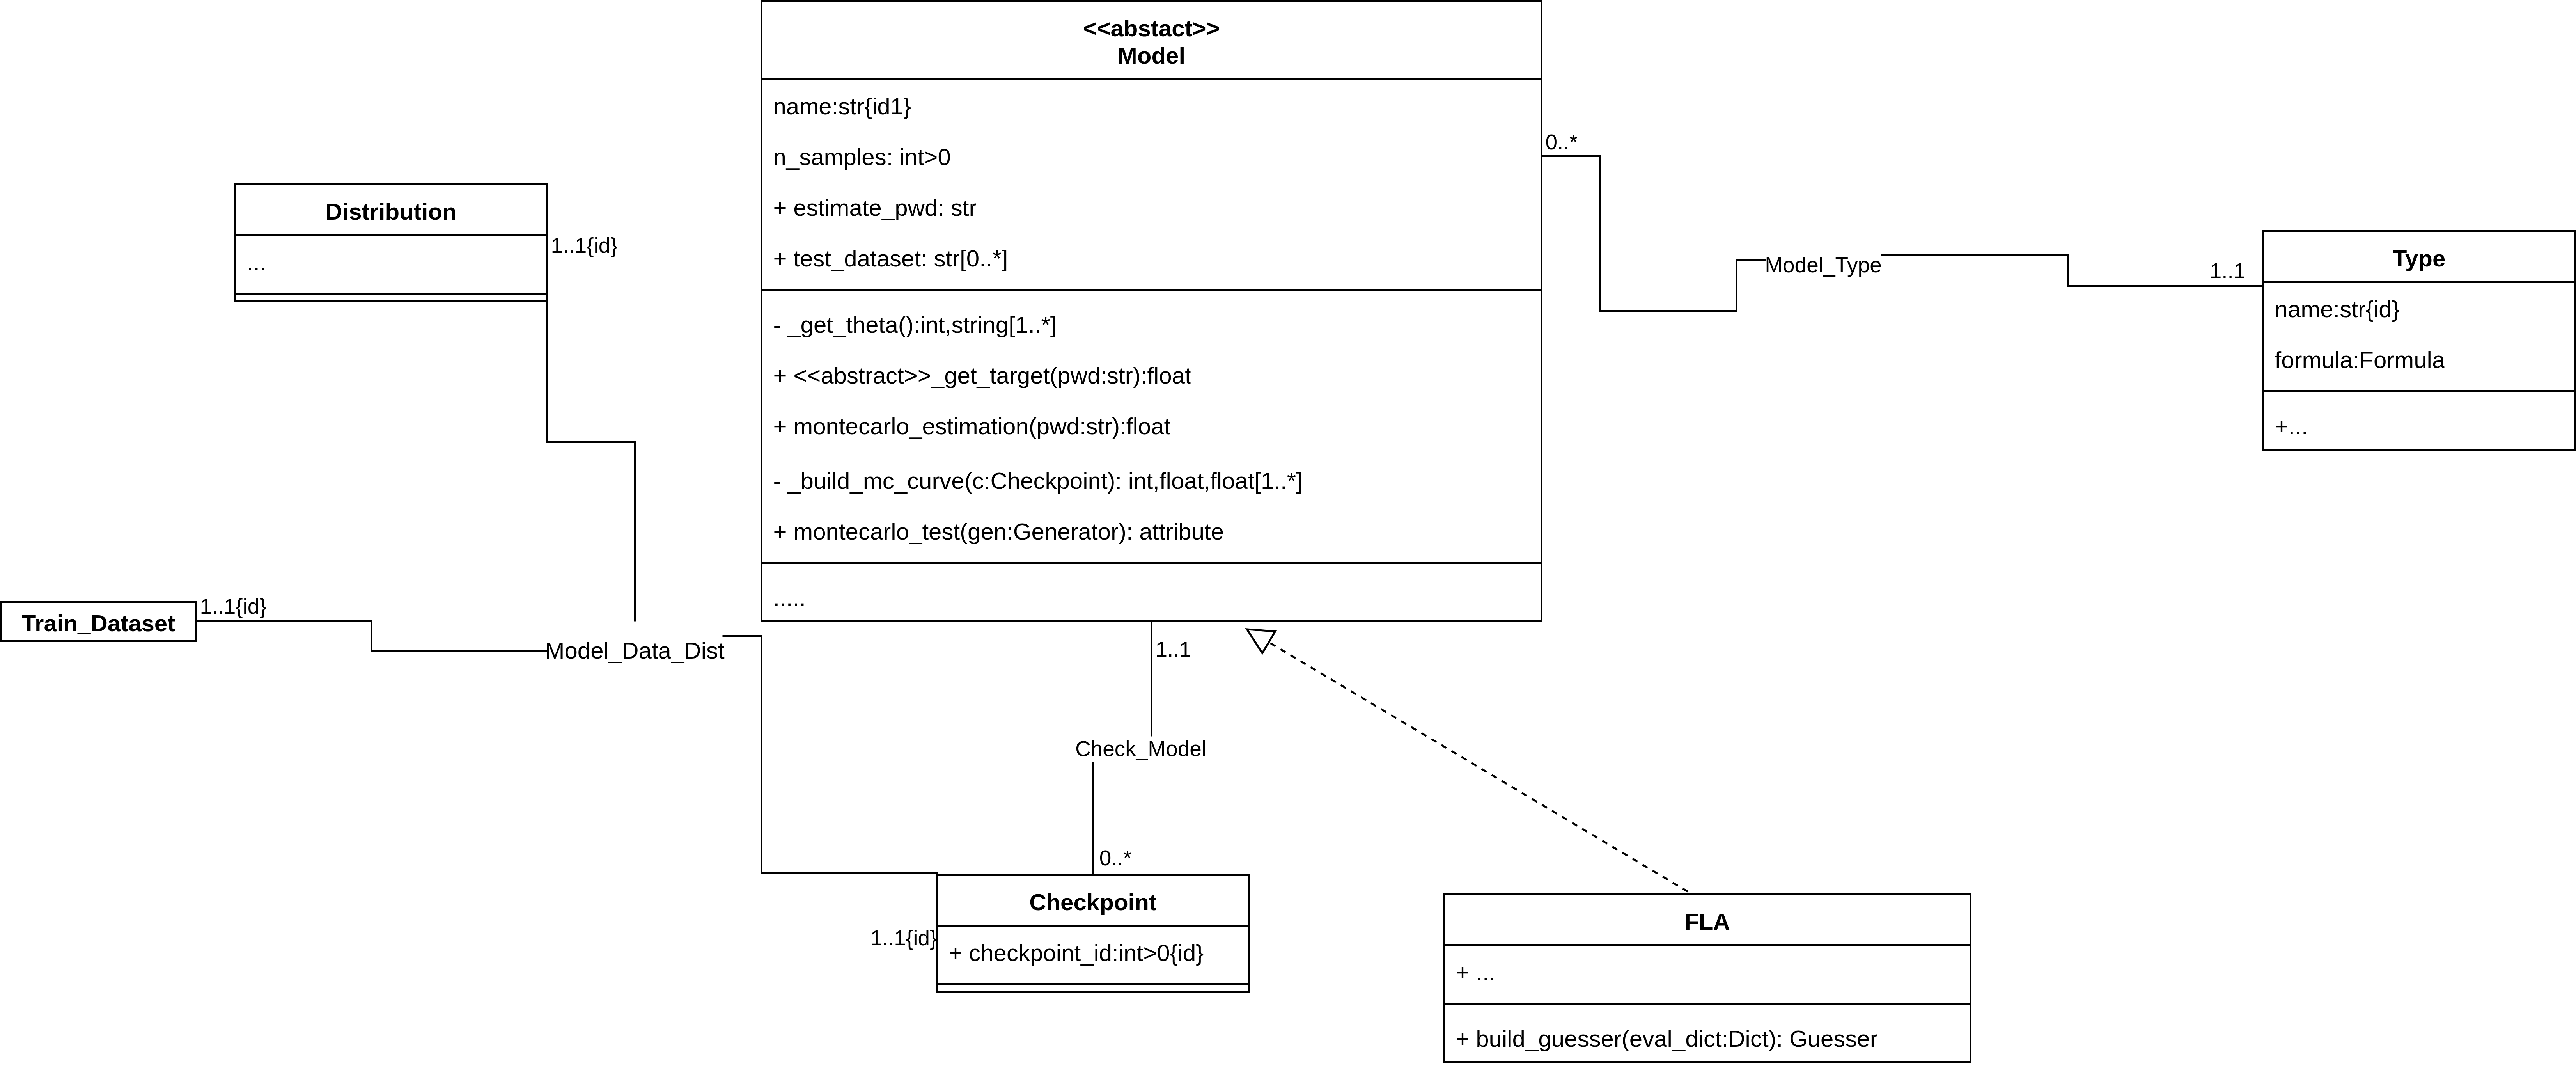
\includegraphics[width=1\linewidth, height=0.4\textheight]{img/UML.png}
    \caption{Analysis}
    \label{fig:uml}
\end{figure}
\FloatBarrier

\section{Extended FOL}
\label{fol}
\begin{align*}
\text{Let }\mathbf{A} := \{(i, prob)  \mid i\in \mathbb{N} \wedge\ (x,prob) \in  sorted(\{x,p \mid \exists pwd \in \Theta\ \wedge x\in \mathbb{N}\\ \wedge\ P(pwd,p)\ \wedge\ x = x +1 \},sort\_func) \wedge i = |\mathbf{A}| +1\} \eqref{eq:rhatopt}
\end{align*}

\begin{align*}
    sort\_func&(t_1:int\geq0,real(0..1),t_2:int\geq0,real(0..1)))\rightarrow Bool:\\
    &preconditions:None\\
    &postconditions:\\
    &|ret := \forall\ n_1,n_2,\\
    &|Real(t_1,n_1) \wedge Real(t_2,n_2) \implies n_1 > n_2\\
    &|\text{return ret}
\end{align*}
%TODO check correctness of this formula, i feel like there is something wrong
\begin{align*}
    \text{Let }\mathbf{C}:= \{(i,n) \mid \exists x,prob \wedge i \in \mathbb{N} \wedge  n \in \mathbb{R}_{>0}  \wedge |A| > 0\wedge n = \frac{1}{|A|}\cdot \sum_{x,prob \in A}^{i\leq x} {\frac{1}{prob}} \} 
\end{align*}

\backmatter
\phantomsection
% This tells LaTeX which style to use. 
% The 'sapthesis' class document
\bibliographystyle{sapthesis} 

% This tells LaTeX to use the .bib file you just created.
% (If you named it "references.bib", use "references")
\bibliography{refs}

\section{Acknowledgements}
"Don’t be overwise; fling yourself straight into life, without deliberation; don’t be afraid - the flood will bear you to the bank and set you safe on your feet again." Fyodor Dostoevsky

\end{document}
